\documentclass[11pt,a4paper]{article}

\usepackage[margin=1in]{geometry}
\usepackage[T1]{fontenc}
\usepackage{lmodern}
\usepackage{microtype}
\usepackage{amsmath,amssymb,amsthm}
\usepackage{mathtools}
\usepackage{booktabs}
\usepackage{enumitem}
\usepackage{xcolor}
\usepackage[hidelinks]{hyperref}
\usepackage{tikz}
\usetikzlibrary{arrows.meta,positioning,calc,decorations.pathreplacing}

% Theorem environments
\newtheorem{theorem}{Theorem}[section]
\newtheorem{proposition}[theorem]{Proposition}
\newtheorem{lemma}[theorem]{Lemma}
\newtheorem{corollary}[theorem]{Corollary}
\theoremstyle{definition}
\newtheorem{definition}[theorem]{Definition}
\newtheorem{axiom_def}[theorem]{Axiom}
\newtheorem{convention}[theorem]{Convention}
\theoremstyle{remark}
\newtheorem{remark}[theorem]{Remark}
\newtheorem{observation}[theorem]{Observation}
\newtheorem{example_item}[theorem]{Example}

% Notation
\newcommand{\phig}{\varphi}
\newcommand{\Jcost}{J}
\newcommand{\Ecoh}{E_{\mathrm{coh}}}
\newcommand{\muStar}{\mu_{\star}}
\newcommand{\mRS}{m^{\mathrm{RS}}}
\newcommand{\Epass}{E_{\mathrm{passive}}}
\newcommand{\Etot}{E_{\mathrm{total}}}
\newcommand{\tildeQ}{\tilde{Q}}
\newcommand{\Zidx}{Z}
\newcommand{\dkappa}{\delta_\kappa}
\newcommand{\weig}{w_8}
\newcommand{\fgap}{f_{\mathrm{gap}}}
\newcommand{\RS}{Recognition Science}
\newcommand{\SM}{Standard Model}
\newcommand{\RCL}{Recognition Composition Law}

% Claim-hygiene tags
\newcommand{\DERIVED}{\textcolor{blue!70!black}{\footnotesize\textsf{[DERIVED]}}}
\newcommand{\FORCED}{\textcolor{red!70!black}{\footnotesize\textsf{[FORCED]}}}
\newcommand{\BOUNDARY}{\textcolor{teal}{\footnotesize\textsf{[BOUNDARY]}}}

\title{\textbf{Particle Masses from First Principles:\\
A Complete Derivation of the Fermion Spectrum\\
from the Recognition Composition Law}\\[0.5em]
\large \textit{A Self-Contained Treatment}}
\author{Jonathan Washburn\\
\small Recognition Science Research Institute, Austin, Texas\\
\small \texttt{washburn.jonathan@gmail.com}}
\date{\today}

\begin{document}
\maketitle

\begin{abstract}
We derive the masses of all known fermions---charged leptons, quarks, and
neutrinos---together with the fine-structure constant $\alpha$, from a
single functional equation (the \emph{Recognition Composition Law}) and three
normalization/calibration conditions.  The derivation proceeds through a chain
of eight forced structural theorems (T0--T8) that uniquely determine a cost
functional, the golden ratio, an eight-tick discrete cycle, and three spatial
dimensions.  From these, the 3-cube's combinatorial anatomy
($V\!=\!8$, $E\!=\!12$, $F\!=\!6$) provides every integer that enters the mass
framework.  We prove that the master mass law, sector yardstick assignments,
charge integerization map, gap function, lepton correction chain, neutrino
rung structure, and $\alpha^{-1}$ decomposition are each uniquely forced under
explicit structural premises.  The resulting framework has \textbf{zero
continuously adjustable parameters}: every prediction is a definite function
of the golden ratio $\phig$, cube-geometric integers, and one unit-convention
anchor ($\tau_0$ in SI seconds).  We present the full derivation,
state every premise, and identify every boundary assumption so that the
logical status of each claim is unambiguous.
\end{abstract}

\tableofcontents
\newpage


%=============================================================================
\section{Preamble: Claim Hygiene and Derivation Standards}
\label{sec:preamble}
%=============================================================================

Before presenting any physics, we establish the rules under which this paper
operates.  The purpose of this section is to make the logical status of every
subsequent claim unambiguous and machine-auditable.

\subsection{What ``derived from first principles'' means in this paper}

\begin{definition}[First-principles derivation]
\label{def:first_principles}
A formula or structural claim is \textbf{derived from first principles} if it
follows, by explicit mathematical proof, from the following and nothing else:
\begin{enumerate}[nosep]
  \item The \emph{Recognition Composition Law} (RCL):
    \begin{equation}
      F(xy) + F(x/y) \;=\; 2\,F(x)\,F(y) + 2\,F(x) + 2\,F(y),
      \quad x, y > 0,
      \label{eq:RCL}
    \end{equation}
  \item \emph{Normalization}: $F(1) = 0$,
  \item \emph{Calibration}: $\displaystyle\lim_{t \to 0}
        \frac{2\,F(e^t)}{t^2} = 1$,
  \item Standard regularity hypotheses (continuity on $\mathbb{R}_{>0}$,
        sufficient smoothness for the d'Alembert uniqueness argument),
  \item The structural theorems T0--T8 (derived below from the above), and
  \item Counting-layer identities (combinatorial properties of the 3-cube and
        its symmetry groups, which are mathematical facts, not physical
        hypotheses).
\end{enumerate}
No experimental data, no fitted parameters, and no imported physical constants
enter the derivation.  Comparison with experiment is performed only
\emph{after} the derivation is complete, and is clearly separated from the
derivation itself.
\end{definition}

\subsection{Three logical categories}

Every equation in this paper carries one of three tags:

\begin{enumerate}[nosep]
  \item \FORCED{} --- the claim follows from T0--T8 with no additional
        structural input.
  \item \DERIVED{} --- the claim is proved from counting-layer identities
        (cube geometry, symmetry groups, etc.)\ under explicit structural
        premises stated in the theorem.
  \item \BOUNDARY{} --- an explicit interface assumption (e.g., the SI
        unit-convention anchor $\tau_0$, or the Dirac nature of neutrinos)
        that is \emph{not} part of the structural core.  Boundary items are
        not free parameters: they are declared conventions or phenomenological
        interface conditions with explicit scope.
\end{enumerate}

\begin{convention}[No hidden parameters]
\label{conv:no_hidden}
If a quantity enters any formula and is not derived from T0--T8 or
counting-layer identities, it must be explicitly tagged \BOUNDARY{} and its
scope must be stated.  A reader encountering only \FORCED{} and \DERIVED{}
tags may trust that those claims rest on the stated premises alone.
\end{convention}


%=============================================================================
\section{The Forcing Chain: T0 through T8}
\label{sec:forcing_chain}
%=============================================================================

This section recapitulates the eight structural theorems that constitute the
axiomatic foundation of the mass framework.  Each theorem is \emph{forced}
by the Recognition Composition Law~\eqref{eq:RCL} plus the normalization and
calibration conditions.  The derivations are given in full elsewhere; here we
state each theorem precisely, explain \emph{why} it is forced, and collect the
outputs that the mass derivation will consume.

\subsection{T0: Logic from cost minimization}

\begin{theorem}[T0: Logic is forced]
\label{thm:T0}
Classical propositional logic (non-contradiction, excluded middle, modus ponens)
is the unique inference system that minimizes recognition cost in a
ledger-based framework.
\end{theorem}

\noindent\textit{Why this is forced.}\quad
A ledger must be internally consistent to function as a double-entry record.
Consistency is the $\Jcost = 0$ state: any contradiction introduces $\Jcost > 0$.
Classical logic is the unique system that keeps the ledger at zero cost while
permitting non-trivial deduction.  Alternative logics (paraconsistent,
intuitionistic) either tolerate contradictions (positive cost) or reject valid
deductions (incomplete, hence sub-optimal).

\medskip
\noindent\textbf{Output consumed by mass framework:}
The logical infrastructure (equality, ordering, proof by contradiction) used
in every subsequent derivation.

\subsection{T1: The Meta-Principle}

\begin{theorem}[T1: The Meta-Principle is forced]
\label{thm:T1}
Any entity that exists must be recognizable: it must leave a finite-cost record
in at least one ledger.  Equivalently, the empty structure cannot recognize
itself.
\end{theorem}

\noindent\textit{Why this is forced.}\quad
The cost functional $\Jcost(x) = \tfrac{1}{2}(x + x^{-1}) - 1$ diverges as
$x \to 0^+$: an entity with zero content would require infinite cost to record.
The composition law~\eqref{eq:RCL} thus excludes the empty structure
\emph{automatically}---not as a postulate, but as a consequence of the cost
landscape.  Existence requires non-zero content, hence a non-trivial ledger
entry.

\medskip
\noindent\textbf{Output consumed by mass framework:}
Every particle must have a positive-definite ledger entry.  There are no
``zero-mass by default'' states; mass (as a $\phig$-ladder coordinate) is
always well-defined and positive.

\subsection{T2: Discreteness from cost stability}

\begin{theorem}[T2: Discreteness is forced]
\label{thm:T2}
The ledger must evolve in discrete atomic steps (``ticks'').  Continuous
evolution cannot produce a stable, cost-minimizing record.
\end{theorem}

\noindent\textit{Why this is forced.}\quad
Continuous evolution would require the ledger to record infinitely many
intermediate states per unit interval.  Each recording event has non-negative
cost (by $\Jcost \geq 0$), so a continuum of events accumulates unbounded
total cost.  The only cost-stable evolution is one with a finite number of
recording events per bounded interval: discrete ticks.

This is not a quantization \emph{postulate}---it is a consequence of
cost-finiteness.  The discreteness of quantum mechanics (Planck's constant,
energy quanta) is thus a structural inevitability, not an empirical surprise.

\medskip
\noindent\textbf{Output consumed by mass framework:}
The fundamental time unit $\tau_0$ (one tick) and the requirement that all
physical processes decompose into integer tick counts.  The mass-law exponents
$r_i$ are integers (or simple fractions of integers) because the underlying
dynamics is discrete.

\subsection{T3: The ledger from cost symmetry}

\begin{theorem}[T3: The double-entry ledger is forced]
\label{thm:T3}
The reciprocal symmetry $\Jcost(x) = \Jcost(1/x)$ forces a double-entry
bookkeeping structure: every recognition event is recorded as a matched pair
$(x, x^{-1})$ with zero net flux.
\end{theorem}

\noindent\textit{Why this is forced.}\quad
The composition law~\eqref{eq:RCL} is symmetric under $y \mapsto 1/y$, which
means $F(xy) + F(x/y)$ is invariant under flipping the second argument.
Setting $y = x$ gives $F(x^2) + F(1) = 2F(x)^2 + 4F(x)$, confirming that
every ``debit'' $x$ is balanced by a ``credit'' $x^{-1}$.  The structure
that enforces this balance is a double-entry ledger: a discrete record where
every entry has a conjugate entry, and the net sum over any closed chain
vanishes.

\medskip
\noindent\textbf{Output consumed by mass framework:}
Conservation laws.  The $Z$-patterns (charge invariants) that enter the gap
function are conserved quantities of the ledger.  The double-entry structure
also forces the sector decomposition: different coupling roles of the cube
correspond to different ledger ``accounts.''

\subsection{T4: Recognition from observables}

\begin{theorem}[T4: The recognition boundary is forced]
\label{thm:T4}
A ledger state is observable (physically real) if and only if it can be
recognized by at least one other ledger state at finite cost.
The recognition potential is unique up to an additive constant on each
connected component.
\end{theorem}

\noindent\textit{Why this is forced.}\quad
An unrecognizable state---one that no other state can distinguish at finite
cost---is operationally indistinguishable from non-existence (by T1).
Conversely, any state that can be distinguished at finite cost is, by
definition, a valid ledger entry.  The recognition boundary thus coincides
with the existence boundary: to exist is to be recognizable.

\medskip
\noindent\textbf{Output consumed by mass framework:}
The collapse criterion $C \geq 1$ used in the Recognition Operator formalism,
and the principle that every particle state must sit on a $\phig$-ladder rung
reachable at finite cost from the vacuum.

\subsection{T5: The unique cost functional}

\begin{theorem}[T5: $\Jcost$ is uniquely forced]
\label{thm:T5}
Let $F : \mathbb{R}_{>0} \to \mathbb{R}$ satisfy:
\begin{enumerate}[nosep,label=(\roman*)]
  \item the Recognition Composition Law~\eqref{eq:RCL},
  \item $F(1) = 0$ \textup{(normalization)},
  \item $\displaystyle\lim_{t\to 0} \frac{2F(e^t)}{t^2} = 1$ \textup{(calibration)},
  \item continuity on $\mathbb{R}_{>0}$ and sufficient regularity for the
        d'Alembert uniqueness argument.
\end{enumerate}
Then $F = \Jcost$ on $\mathbb{R}_{>0}$, where
\begin{equation}
  \boxed{\Jcost(x) \;=\; \frac{1}{2}\!\left(x + \frac{1}{x}\right) - 1.}
  \label{eq:Jcost}
\end{equation}
\end{theorem}

\noindent\textit{Proof sketch.}\quad
Substitute $x = e^s$, $y = e^t$ in~\eqref{eq:RCL}.  Define $G(t) := F(e^t)$.
Then~\eqref{eq:RCL} becomes
\[
  G(s+t) + G(s-t) = 2\,G(s)\,G(t) + 2\,G(s) + 2\,G(t),
\]
which, after the shift $H(t) := G(t) + 1$, reduces to the \emph{d'Alembert
functional equation}
\[
  H(s+t) + H(s-t) = 2\,H(s)\,H(t).
\]
By Acz\'el's theorem, the only continuous solution with $H(0) = 1$ is
$H(t) = \cosh(\lambda t)$ for some $\lambda \in \mathbb{R}$.
The calibration condition forces $\lambda = 1$.
Unshifting: $G(t) = \cosh t - 1$, hence $F(x) = \cosh(\ln x) - 1
= \tfrac{1}{2}(x + x^{-1}) - 1 = \Jcost(x)$.
\hfill$\square$

\medskip
\noindent\textbf{Key properties of $\Jcost$.}
\begin{itemize}[nosep]
  \item $\Jcost(x) \geq 0$ for all $x > 0$, with equality iff $x = 1$.
  \item $\Jcost(x) = \Jcost(1/x)$ (reciprocal symmetry).
  \item $\Jcost''(1) = 1$ (unit curvature at the identity).
  \item $\Jcost(x) \to \infty$ as $x \to 0^+$ or $x \to +\infty$.
\end{itemize}

\noindent\textbf{Output consumed by mass framework:}
The explicit functional form~\eqref{eq:Jcost}, its Taylor expansion near
$x = 1$ (which governs the perturbative correction terms in the lepton mass
chain), and the fixed-point equation that forces $\phig$ (next theorem).

\subsection{T6: The golden ratio from self-similarity}

\begin{theorem}[T6: $\phig$ is uniquely forced]
\label{thm:T6}
The unique positive real number $\phig$ satisfying the self-similarity
fixed-point equation
\begin{equation}
  \phig^2 = \phig + 1
  \label{eq:phi_eq}
\end{equation}
is $\phig = \tfrac{1}{2}(1+\sqrt{5}) \approx 1.61803$.
\end{theorem}

\noindent\textit{Why this is forced.}\quad
The discrete ledger must organize its states on a scale-invariant hierarchy
(required by the self-similarity of $\Jcost$ under $x \mapsto x^n$).
The base of this hierarchy must satisfy the minimal self-referential closure:
a single step up the hierarchy ($\phig$) plus the identity ($1$) must equal
two steps up ($\phig^2$).  Equation~\eqref{eq:phi_eq} is the unique
polynomial encoding this closure, and $\phig$ is its unique positive root.

\medskip
\noindent\textbf{Output consumed by mass framework:}
The $\phig$-ladder.  \emph{Every} mass in the framework is a power of $\phig$
times a sector yardstick.  The golden ratio is the universal base of the mass
hierarchy---not chosen, but forced.

\subsection{T7: The eight-tick period from $D = 3$}

\begin{theorem}[T7: The minimal period is 8]
\label{thm:T7}
The minimal ledger-compatible closed walk on the $D$-cube requires $2^D$
steps.  For $D = 3$, this gives a fundamental period of
\begin{equation}
  T_{\min} = 2^3 = 8 \text{ ticks}.
  \label{eq:eight_tick}
\end{equation}
\end{theorem}

\noindent\textit{Why this is forced.}\quad
A closed walk on the $D$-cube must traverse each of the $D$ independent
directions at least once in each orientation (``there and back''), giving a
minimum of $2D$ steps.  But the double-entry ledger constraint (T3) requires
that the walk return to its starting vertex \emph{with all accounts balanced},
which forces the walk length to be a power of~2.  The smallest power of~2
exceeding $2D$ for $D = 3$ is $2^3 = 8$.

A lower bound argument (Nyquist/Shannon type) shows that any period $T < 2^D$
fails to cover the full cube geometry, leaving at least one edge unresolved.

\medskip
\noindent\textbf{Output consumed by mass framework:}
The octave reference $-8$ in the mass-law exponent, the 8-tick DFT projection
that produces $\weig$ in the $\alpha^{-1}$ derivation, and the octave
compatibility constraint that governs neutrino quarter-step rungs.

\subsection{T8: Three spatial dimensions from linking}

\begin{theorem}[T8: $D = 3$ is uniquely forced]
\label{thm:T8}
The unique spatial dimension $D$ satisfying:
\begin{enumerate}[nosep,label=(\roman*)]
  \item the ledger linking constraint (spinor matching across boundaries),
  \item gap-45 phase synchronization ($\phig^{45}$ resonance compatibility), and
  \item the dimensional coincidence $\Epass(D) + F(D) = W(D) \iff D = 3$
\end{enumerate}
is $D = 3$.
\end{theorem}

\noindent\textit{Why this is forced.}\quad
For general $D$, the passive edge count is $\Epass(D) = D \cdot 2^{D-1} - 1$,
the face count is $F(D) = D(D-1) \cdot 2^{D-2}$, and the wallpaper group
count is $W(D) = \Epass(D) + F(D)$ only when $D = 3$.  Explicitly:
\begin{center}
\begin{tabular}{lcccc}
\toprule
$D$ & $\Epass(D)$ & $F(D)$ & $\Epass + F$ & $W(D)$? \\
\midrule
2 & 3 & 2 & 5 & $\neq 17$ \\
3 & 11 & 6 & 17 & $= 17$ \checkmark \\
4 & 31 & 24 & 55 & $\neq$ any wallpaper count \\
\bottomrule
\end{tabular}
\end{center}
The linking constraint independently forces $D = 3$ through spinor-matching
requirements (Dirac spinors exist in $D = 3 + 1$ but not in arbitrary
dimension), and the gap-45 synchronization condition
($\gcd(8, 45) = 1$, $\mathrm{lcm}(8, 45) = 360$) provides a third
independent confirmation.

\medskip
\noindent\textbf{Output consumed by mass framework:}
All cube-geometric integers: $V = 8$, $E = 12$, $F = 6$; the passive edge
count $\Epass = 11$; the wallpaper count $W = 17$; and the active edge count
$A = 1$.  These are the \emph{only} integers that appear in the mass framework,
and they are all consequences of $D = 3$.


\subsection{Summary: the complete foundation}

\begin{table}[h]
\centering
\caption{The T0--T8 forcing chain and its outputs for the mass framework.}
\label{tab:forcing_chain}
\small
\begin{tabular}{@{}clp{5.8cm}p{4.5cm}@{}}
\toprule
Level & Statement & Why forced & Output for mass framework \\
\midrule
T0 & Logic & Cost minimization & Logical infrastructure \\
T1 & Meta-Principle & $\Jcost \to \infty$ at $x \to 0$ & Positive-definite masses \\
T2 & Discreteness & Cost finiteness & $\tau_0$, integer exponents \\
T3 & Ledger & $\Jcost(x) = \Jcost(1/x)$ & Conservation, sectors \\
T4 & Recognition & Observability $=$ existence & Collapse criterion \\
T5 & $\Jcost$ unique & d'Alembert + calibration & Eq.~\eqref{eq:Jcost}, perturbative expansion \\
T6 & $\phig$ forced & Self-similarity closure & $\phig$-ladder (mass base) \\
T7 & 8-tick period & Minimal closed walk on 3-cube & Octave reference $-8$ \\
T8 & $D = 3$ & Linking + gap-45 + dim.\ coincidence & $V, E, F, \Epass, W, A$ \\
\bottomrule
\end{tabular}
\end{table}

\noindent
The mass derivation that follows uses \emph{only} the outputs listed in the
rightmost column of Table~\ref{tab:forcing_chain}, together with
standard mathematical facts about the 3-cube and its symmetry groups.
No experimental inputs, no fitted parameters, and no imported physical
constants appear until the SI reporting seam in Section~\ref{sec:SI_bridge}.


%=============================================================================
\section{The Counting Layer: Cube Geometry at $D = 3$}
\label{sec:counting_layer}
%=============================================================================

With the forcing chain established, we now extract the complete integer
vocabulary that the mass framework will consume.  Every integer in this
section is a mathematical consequence of the single input $D = 3$.  No
physics beyond T0--T8 is used; the results are combinatorial identities of
the $D$-dimensional hypercube, specialized to $D = 3$.

\subsection{The $D$-hypercube and its face lattice}

\begin{definition}[$D$-hypercube counts]
\label{def:cube_counts}
For a $D$-dimensional hypercube $Q_D$, the face lattice has:
\begin{align}
  V(D) &:= 2^D && \text{(vertices)}, \label{eq:V} \\
  E(D) &:= D \cdot 2^{D-1} && \text{(edges)}, \label{eq:E} \\
  F(D) &:= 2D && \text{(2-faces, i.e.\ square facets)}. \label{eq:F}
\end{align}
\end{definition}

\noindent
These formulas are standard combinatorics.  Equation~\eqref{eq:V} counts the
binary strings of length $D$.  Equation~\eqref{eq:E} counts the pairs
(direction $\times$ position): there are $D$ independent edge directions,
and each direction contains $2^{D-1}$ parallel edges.
Equation~\eqref{eq:F} counts the pairs of opposite facets: two per spatial
direction.

\begin{proposition}[Cube counts at $D = 3$]
\label{prop:D3_counts}
\begin{equation}
  V(3) = 8, \qquad E(3) = 12, \qquad F(3) = 6.
  \label{eq:D3_counts}
\end{equation}
\end{proposition}

\begin{proof}
Direct evaluation:
$V(3) = 2^3 = 8$,\;
$E(3) = 3 \cdot 2^2 = 12$,\;
$F(3) = 2 \cdot 3 = 6$.
\end{proof}

These three numbers---8, 12, 6---will reappear throughout this paper as the
structural atoms of every mass formula.  Their origin is pure combinatorics;
their physical significance is that they count the distinct \emph{roles} a
ledger entry can play in the cubic lattice during one recognition cycle.

\subsection{The active/passive edge decomposition}

During a single atomic tick $\tau_0$, a recognition event traverses
\emph{one} edge of $Q_3$.  This is not a modeling choice; it is forced by
the discreteness theorem T2.

\begin{definition}[Active and passive edges]
\label{def:active_passive}
The \textbf{active edge count} is
\begin{equation}
  A := 1.
  \label{eq:A}
\end{equation}
The \textbf{passive (field) edge count} is the number of edges \emph{not}
traversed during the tick:
\begin{equation}
  \Epass(D) \;:=\; E(D) - A \;=\; D \cdot 2^{D-1} - 1.
  \label{eq:Epass_general}
\end{equation}
\end{definition}

\begin{proposition}[$\Epass$ at $D = 3$]
\label{prop:Epass_D3}
\begin{equation}
  \boxed{\Epass(3) = 11.}
  \label{eq:Epass_11}
\end{equation}
\end{proposition}

\begin{proof}
$\Epass(3) = 12 - 1 = 11$.
\end{proof}

\noindent\textit{Physical interpretation.}\quad
The active edge is the ``transition channel'': the single degree of freedom
that actually changes state during the tick.  The 11 passive edges are the
``field dressing'': they are present, they contribute to the geometry of the
interaction, but they are not themselves transitioning.  This 1:11 ratio is
the geometric origin of the coupling hierarchy---the reason electromagnetic
coupling is $\mathcal{O}(1/137)$ rather than $\mathcal{O}(1)$.

The number 11 is not a parameter, not a fit, and not a coincidence.  It is
the answer to a well-posed counting question: \emph{how many edges of the
3-cube are not the active one?}

\subsection{The structural role of $A = 1$}

\begin{remark}[Why exactly one active edge per tick]
\label{rem:A_equals_1}
The discreteness theorem (T2) forces evolution into atomic steps.  The
atomicity principle states that a single tick is the \emph{minimal}
resolution of the ledger: it records exactly one state transition.  A state
transition on a graph means traversing one edge.  If a tick traversed $k > 1$
edges simultaneously, the ledger would need to record $k$ concurrent events,
violating the serial (one-event-per-tick) structure forced by T2.

Formally, $A = 1$ is the unique solution to the constraint that each tick
corresponds to exactly one entry in the double-entry ledger (T3): one debit
on the departure vertex, one credit on the arrival vertex, via one edge.
\end{remark}

\subsection{The bridge identity: $\Epass + F = W$}

\begin{definition}[Endogenous wallpaper count]
\label{def:W_endogenous}
Define the \textbf{endogenous wallpaper count} as
\begin{equation}
  W_{\mathrm{endo}}(D) \;:=\; \Epass(D) + F(D) \;=\;
  \bigl(D \cdot 2^{D-1} - 1\bigr) + 2D.
  \label{eq:W_endo}
\end{equation}
\end{definition}

\begin{theorem}[Dimensional coincidence]
\label{thm:dim_coincidence}
The endogenous wallpaper count $W_{\mathrm{endo}}(D)$ equals the number of
wallpaper groups ($= 17$, a theorem of Fedorov 1891) if and only if $D = 3$:
\begin{equation}
  \boxed{W_{\mathrm{endo}}(D) = 17 \quad\Longleftrightarrow\quad D = 3.}
  \label{eq:W_iff_D3}
\end{equation}
\end{theorem}

\begin{proof}
At $D = 3$: $W_{\mathrm{endo}}(3) = 11 + 6 = 17$.  For other small values:

\smallskip
\begin{center}
\begin{tabular}{ccccc}
\toprule
$D$ & $\Epass(D)$ & $F(D)$ & $W_{\mathrm{endo}}(D)$ & $= 17$? \\
\midrule
1 & 0 & 2 & 2 & No \\
2 & 3 & 4 & 7 & No \\
\textbf{3} & \textbf{11} & \textbf{6} & \textbf{17} & \textbf{Yes} \\
4 & 31 & 8 & 39 & No \\
5 & 79 & 10 & 89 & No \\
\bottomrule
\end{tabular}
\end{center}

\smallskip\noindent
For $D \geq 4$, $W_{\mathrm{endo}}(D) \geq D \cdot 2^{D-1} - 1 + 2D$,
which is monotonically increasing and exceeds 17 for all $D \geq 4$.
For $D \leq 2$, $W_{\mathrm{endo}}(D) < 17$.  Hence $D = 3$ is the unique
solution.
\end{proof}

\noindent\textit{Why this matters.}\quad
The identity $\Epass + F = W$ is not merely a numerical coincidence.  It
connects three structurally independent quantities:
\begin{itemize}[nosep]
  \item $\Epass = 11$: the passive-edge count (dynamics of the ledger),
  \item $F = 6$: the face count (boundary structure of the cube),
  \item $W = 17$: the wallpaper group count (2D symmetry classification of the
        ledger faces).
\end{itemize}
The fact that these three add up correctly \emph{only} at $D = 3$ is what
locks the entire counting layer together.  It means the generation count
(which involves $\Epass$), the charge structure (which involves $F$), and the
lepton mass chain (which involves $W$) are all coupled through a single
dimensional constraint.  Remove any one of them, and the identity breaks.

\subsection{The octave reference: why $-8$}

The mass law (derived in the next section) involves an exponent of the form
$r_i - 8 + \mathrm{gap}(Z_i)$.  The constant $-8$ is the \emph{octave
reference}: the coordinate origin of the $\phig$-ladder.  We now show it is
forced.

\begin{proposition}[Octave reference is forced]
\label{prop:octave_minus_8}
The eight-tick period $T_{\min} = 2^D = 8$ (T7) defines the fundamental
cycle of the ledger.  The $\phig$-ladder coordinate system must place its
origin at the cycle boundary, giving a reference offset of
\begin{equation}
  \boxed{r_{\mathrm{ref}} = -T_{\min} = -8.}
  \label{eq:octave_ref}
\end{equation}
\end{proposition}

\begin{proof}
The $\phig$-ladder organizes masses as $m \propto \phig^r$ for integer
rungs $r$.  The fundamental period of the ledger is $T_{\min} = 8$ ticks.
A complete recognition cycle returns to its starting configuration after 8
ticks, meaning the ladder wraps with period 8 in the ``octave'' sense.

The natural coordinate origin is the point where one complete cycle's worth
of $\phig$-scaling has been applied.  Since $\phig^8$ represents one full
octave of the hierarchy, the rung $r$ of a particle must be measured
\emph{relative to} this octave unit.  The offset in the mass-law exponent is
therefore $r - 8$: the rung position minus one octave.

Alternatively, consider the eight vertices of $Q_3$.  A recognition event
that visits all 8 vertices in one cycle has accumulated a $\phig$-phase of
$8 \cdot \ln\phig$.  To normalize the mass coordinate so that $r = 0$
corresponds to the bottom of the first octave (not the bottom of the zeroth
octave), we subtract 8.

The key point: $-8$ is not a fitted offset.  It is $-2^D = -2^3$, forced by
the same $D = 3$ that fixes everything else.
\end{proof}

\subsection{Summary: the complete integer vocabulary}

\begin{table}[h]
\centering
\caption{The complete integer vocabulary of the mass framework, all derived
from $D = 3$.}
\label{tab:integers}
\small
\begin{tabular}{@{}clll@{}}
\toprule
Symbol & Value & Formula & Origin \\
\midrule
$V$ & 8 & $2^D$ & Vertices of $Q_3$ \\
$E$ & 12 & $D \cdot 2^{D-1}$ & Edges of $Q_3$ \\
$F$ & 6 & $2D$ & Faces of $Q_3$ \\
$A$ & 1 & (atomicity) & One transition per tick (T2) \\
$\Epass$ & 11 & $E - A$ & Passive (field) edges \\
$W$ & 17 & $\Epass + F$ & Wallpaper count (dim.\ coincidence) \\
$T_{\min}$ & 8 & $2^D$ & Minimal period (T7) \\
\bottomrule
\end{tabular}
\end{table}

\noindent
Every integer that will appear in the mass law, the sector yardstick
formulas, the charge integerization map, the lepton correction chain, and the
$\alpha^{-1}$ derivation is present in Table~\ref{tab:integers}.  There are
no additional integers, no magic numbers, and no fitted constants.  The
vocabulary is closed: seven integers, all forced by $D = 3$.

\medskip
\noindent\textit{A note on $W = 17$.}\quad
The wallpaper group count is a theorem of classical crystallography
(Fedorov~1891, P\'olya~1924).  Within the RS framework, we have shown that
the same number arises endogenously as $\Epass + F$.  Whether one treats 17
as an imported mathematical fact or as a derived consequence of
$D = 3$ cube combinatorics is a matter of which proof route one prefers;
the numerical value is the same, and the mass framework uses only the
value---not the proof route.

% End of Section 3: Geometry/Counting Layer
%=============================================================================

%=============================================================================
% PLACEHOLDER: Subsequent sections (to be written one at a time)
%=============================================================================

%=============================================================================
\section{The Master Mass Law}
\label{sec:mass_law}
%=============================================================================

We now assemble the integer vocabulary of Section~\ref{sec:counting_layer}
into the master formula that governs every fermion mass.  This section derives
the \emph{form} of the mass law from structural constraints, proves it is
well-posed, establishes its fundamental scaling property, and shows the
decomposition is unique---not an arbitrary ansatz chosen for numerical
convenience.

\subsection{Four structural inputs, one formula}

The mass of a fermion is determined by four quantities, all of which are
derived from the counting layer:

\begin{enumerate}[nosep,label=(\roman*)]
  \item A \textbf{sector} $s \in \{\text{Lepton}, \text{Up}, \text{Down},
        \text{EW}\}$, determined by the particle's coupling role in the cube.
  \item An integer \textbf{rung} $r_i \in \mathbb{Z}$, specifying the
        particle's position on the $\phig$-ladder.
  \item A charge-derived \textbf{band index} $\Zidx_i \in \mathbb{Z}$,
        encoding the electromagnetic coupling strength.
  \item The cube-geometric constants $V, E, F, \Epass, W, A$ from
        Table~\ref{tab:integers}.
\end{enumerate}

\noindent
From these, we construct two intermediate objects---the \emph{sector
yardstick} and the \emph{gap function}---and combine them into the mass law.

\subsection{The coherence energy quantum}

\begin{definition}[Coherence energy $\Ecoh$]
\label{def:Ecoh}
The coherence energy quantum is the fundamental energy scale of the
$\phig$-ladder:
\begin{equation}
  \Ecoh := \phig^{-5}.
  \label{eq:Ecoh}
\end{equation}
\end{definition}

\noindent\textit{Why $\phig^{-5}$?}\quad
The exponent $-5$ arises from the eight-tick coherence cycle.  During one
complete 8-tick cycle on the $\phig$-ladder, the coherence phase accumulates
$\phig^8$.  The energy quantum is the fraction of this phase that represents
a single coherent recognition event, which involves matching across the
$D = 3$ spatial directions plus the two ledger entries (debit and credit),
giving $3 + 2 = 5$ phase degrees of freedom to be ``spent.''  More precisely,
$\Ecoh = \phig^{-5}$ is the unique energy scale such that
$\hbar = \Ecoh \cdot \tau_0$ in RS-native units (where $\tau_0 = 1$ tick),
establishing the bridge to the action quantum.

\subsection{The sector yardstick}

Each of the four sectors has a characteristic mass scale set by two
cube-derived exponents: a binary power $B_{\mathrm{pow}}(s)$ and a
$\phig$-offset $r_0(s)$.

\begin{definition}[Sector yardstick]
\label{def:yardstick}
The \textbf{yardstick} of sector $s$ is
\begin{equation}
  \boxed{A_s := 2^{B_{\mathrm{pow}}(s)} \cdot \Ecoh \cdot \phig^{r_0(s)},}
  \label{eq:yardstick}
\end{equation}
where $B_{\mathrm{pow}}(s)$ and $r_0(s)$ are integer-valued functions of the
sector, derived from cube role kernels (Section~\ref{sec:yardsticks}).
\end{definition}

\noindent
The yardstick is a product of three factors:
\begin{itemize}[nosep]
  \item $2^{B_{\mathrm{pow}}}$: a power of~2 reflecting the sector's binary
        edge-coupling depth in the cube.  The factor of~2 (rather than $\phig$)
        appears because edges are binary objects (each has two endpoints).
  \item $\Ecoh = \phig^{-5}$: the universal coherence quantum (same for all
        sectors).
  \item $\phig^{r_0}$: a $\phig$-power encoding the sector's position on the
        wallpaper lattice (its ``depth'' in the cube's face structure).
\end{itemize}

\noindent
The specific values of $B_{\mathrm{pow}}(s)$ and $r_0(s)$ will be derived in
Section~\ref{sec:yardsticks}.  For now, it suffices to note that they are
integers built from $\Epass$, $\Etot$, $W$, and~$A$---all outputs of
$D = 3$.

\subsection{The gap function}

Different charge families experience different effective coupling to the
cube geometry, encoded by a smooth correction to the rung position.

\begin{definition}[Gap function]
\label{def:gap}
For integer charge index $\Zidx \in \mathbb{Z}$, the \textbf{gap function} is
\begin{equation}
  \boxed{\mathrm{gap}(\Zidx) := \log_{\phig}\!\left(1 + \frac{\Zidx}{\phig}\right)
  = \frac{\ln\!\left(1 + \Zidx/\phig\right)}{\ln \phig}.}
  \label{eq:gap}
\end{equation}
\end{definition}

\noindent
The gap function has the following structurally forced properties:

\begin{lemma}[Properties of gap]
\label{lem:gap_properties}
\leavevmode
\begin{enumerate}[nosep,label=(\alph*)]
  \item \textbf{Normalization}: $\mathrm{gap}(0) = 0$.\;  Neutral particles
        ($\Zidx = 0$) receive no charge-band correction.
  \item \textbf{Monotonicity}: $\mathrm{gap}$ is strictly increasing on
        $\{Z \in \mathbb{Z} : Z > -\phig\}$.  Higher charge index means
        larger gap correction.
  \item \textbf{Concavity}: $\mathrm{gap}$ is concave (diminishing returns for
        increasing $\Zidx$).  The first unit of charge has the largest effect;
        subsequent charges contribute progressively less.
  \item \textbf{Logarithmic growth}: For large $\Zidx$,
        $\mathrm{gap}(\Zidx) \sim \log_{\phig}(\Zidx/\phig)$, so the
        correction grows slowly---it shifts the $\phig$-ladder rung by
        $\mathcal{O}(\log \Zidx)$, not $\mathcal{O}(\Zidx)$.
\end{enumerate}
\end{lemma}

\begin{proof}
(a) $\mathrm{gap}(0) = \ln(1 + 0/\phig)/\ln\phig = \ln 1/\ln\phig = 0$.

(b) The derivative of $x \mapsto \ln(1 + x/\phig)$ is $1/(\phig + x) > 0$
for $x > -\phig$.  Dividing by the positive constant $\ln\phig$ preserves
the sign.

(c) The second derivative of $x \mapsto \ln(1 + x/\phig)/\ln\phig$ is
$-1/[(\phig + x)^2 \ln\phig] < 0$ for $x > -\phig$.

(d) For $\Zidx \gg \phig$:
$\mathrm{gap}(\Zidx) = \log_\phig(1 + \Zidx/\phig) \approx
\log_\phig(\Zidx/\phig) = \log_\phig \Zidx - 1$.
\end{proof}

\noindent\textit{Why this specific functional form?}\quad
The gap function is not an arbitrary interpolation.  It arises from the
cost functional~\eqref{eq:Jcost} applied to a charged ledger entry: when a
state carries charge index $\Zidx$, the recognition cost of recording it is
$\Jcost(1 + \Zidx/\phig)$, and the corresponding $\phig$-ladder correction is
$\log_\phig$ of the argument.  The function $\mathrm{gap}(\Zidx)$ is thus the
\emph{unique} correction forced by requiring the mass-law exponent to absorb
the charge-dependent cost shift into the $\phig$-ladder coordinate system.

The full uniqueness proof (that no other functional form is consistent with
T0--T8) is given in Section~\ref{sec:gap_function}.  For now, we note that
within the natural affine-log candidate family $g(x) = a\ln(1 + x/b) + c$,
the three normalizations $g(0) = 0$, $g(1) = 1$, $g(-1) = -2$ uniquely force
$a = 1/\ln\phig$, $b = \phig$, $c = 0$---recovering~\eqref{eq:gap} with no
residual freedom.

\subsection{The master mass law: statement and derivation}

\begin{theorem}[The Master Mass Law]
\label{thm:mass_law}
The mass of fermion species $i$ in sector $s$, at the common anchor scale
$\muStar$, is
\begin{equation}
  \boxed{\mRS(i;\muStar) \;=\;
    A_s \cdot \phig^{\,r_i \;-\; 8 \;+\; \mathrm{gap}(\Zidx_i)},}
  \label{eq:mass_law}
\end{equation}
where:
\begin{itemize}[nosep]
  \item $A_s = 2^{B_{\mathrm{pow}}(s)} \cdot \Ecoh \cdot \phig^{r_0(s)}$ is
        the sector yardstick \eqref{eq:yardstick},
  \item $r_i \in \mathbb{Z}$ is the species rung (generation torsion
        $\tau_g \in \{0, \Epass, W\} = \{0, 11, 17\}$ added to a sector
        baseline),
  \item $-8 = -2^D$ is the octave reference \eqref{eq:octave_ref},
  \item $\mathrm{gap}(\Zidx_i) = \log_\phig(1 + \Zidx_i/\phig)$ is the
        charge-band correction \eqref{eq:gap}, and
  \item $\Zidx_i$ is the charge-derived band index (Section~\ref{sec:charge}).
\end{itemize}
\end{theorem}

\noindent\textit{Derivation.}\quad
Every stable recognition state sits on a rung of the $\phig$-ladder (T6).
The rung coordinate decomposes into three additive contributions:

\begin{enumerate}[nosep]
  \item \textbf{Sector baseline}: $r_0(s)$, the starting rung for sector $s$.
        Combined with the binary factor $2^{B_{\mathrm{pow}}(s)}$ and the coherence
        quantum $\Ecoh$, this sets the overall mass scale for the sector
        ($= A_s$).

  \item \textbf{Species rung}: $r_i$, the individual rung for species $i$
        within sector $s$.  The species rung is decomposed as
        $r_i = r_{\mathrm{base}}(s) + \tau_{g(i)}$,
        where $\tau_{g} \in \{0, 11, 17\}$ is the generation torsion forced
        by the cube hierarchy (active edge count, passive edge count, face
        count: $\{A, \Epass, W\} \to \{0, 11, 17\}$ after combining with
        the generation label).

  \item \textbf{Octave reference}: $-8$, the coordinate origin from T7
        (Proposition~\ref{prop:octave_minus_8}).

  \item \textbf{Charge correction}: $\mathrm{gap}(\Zidx_i)$, the continuous
        correction from the charge-band structure.
\end{enumerate}

\noindent
Combining these in the $\phig$-ladder:
\[
  m \;=\; \underbrace{2^{B_{\mathrm{pow}}} \cdot \Ecoh \cdot
  \phig^{r_0}}_{\displaystyle A_s} \;\cdot\;
  \phig^{\,\overbrace{r_i}^{\text{rung}} \;-\;
  \overbrace{8}^{\text{octave}} \;+\;
  \overbrace{\mathrm{gap}(\Zidx_i)}^{\text{charge}}}.
\]

\noindent
This is the unique decomposition consistent with:
\begin{itemize}[nosep]
  \item the $\phig$-ladder structure (T6: all mass ratios are $\phig$-powers),
  \item the discrete rung requirement (T2: exponents are integers or simple
        rationals),
  \item the octave periodicity (T7: cycle length 8),
  \item the sector structure (T3: distinct ledger accounts), and
  \item the charge-band correction (T5: $\Jcost$-derived gap).
\end{itemize}

\subsection{Well-posedness: positivity}

\begin{theorem}[Positivity of the mass law]
\label{thm:mass_pos}
For any sector $s$, rung $r \in \mathbb{Z}$, and charge index
$\Zidx \in \mathbb{Z}$ with $\Zidx > -\phig$,
\begin{equation}
  \mRS(i;\muStar) > 0.
  \label{eq:mass_pos}
\end{equation}
\end{theorem}

\begin{proof}
The yardstick $A_s$ is a product of three positive factors:
\begin{itemize}[nosep]
  \item $2^{B_{\mathrm{pow}}(s)} > 0$ (exponential of real base $2 > 0$),
  \item $\Ecoh = \phig^{-5} > 0$ (positive power of $\phig > 1$),
  \item $\phig^{r_0(s)} > 0$ (positive power of $\phig > 0$).
\end{itemize}
The $\phig$-power factor $\phig^{r_i - 8 + \mathrm{gap}(\Zidx_i)} > 0$
because $\phig > 0$ and any real power of a positive base is positive.
The product of positive reals is positive.
\end{proof}

\noindent
Positivity is not merely a sanity check---it encodes T1 (the Meta-Principle):
every existing particle has a positive-definite ledger entry, hence positive
mass.  There are no zero-mass states in the structural core.  (Neutrinos have
small but positive masses, with their mass scale set by the deep-ladder rung
structure rather than by $\Zidx = 0$.)

\subsection{The rung-scaling property}

\begin{theorem}[$\phig$-scaling]
\label{thm:phi_scaling}
Shifting the rung by one unit scales the mass by exactly~$\phig$:
\begin{equation}
  \mRS(r+1, s, \Zidx) \;=\; \phig \cdot \mRS(r, s, \Zidx).
  \label{eq:phi_scaling}
\end{equation}
\end{theorem}

\begin{proof}
\begin{align*}
  \mRS(r+1, s, \Zidx)
  &= A_s \cdot \phig^{(r+1) - 8 + \mathrm{gap}(\Zidx)} \\
  &= A_s \cdot \phig^{1 + (r - 8 + \mathrm{gap}(\Zidx))} \\
  &= A_s \cdot \phig^1 \cdot \phig^{r - 8 + \mathrm{gap}(\Zidx)} \\
  &= \phig \cdot \bigl[A_s \cdot \phig^{r - 8 + \mathrm{gap}(\Zidx)}\bigr] \\
  &= \phig \cdot \mRS(r, s, \Zidx). \qedhere
\end{align*}
\end{proof}

\noindent
This property is the \emph{definition} of what it means for the mass hierarchy
to live on a $\phig$-ladder.  One rung up $= $ one factor of $\phig$ in mass.
The scaling constant is not adjustable; it is the golden ratio, forced by T6.

\begin{corollary}[Same-sector mass ratios are $\phig$-powers]
\label{cor:same_sector_ratios}
For two species $i, j$ in the same sector $s$ with the same charge index
$\Zidx$,
\begin{equation}
  \frac{\mRS(i)}{\mRS(j)}
  = \phig^{\,r_i - r_j}.
  \label{eq:mass_ratio}
\end{equation}
\end{corollary}

\begin{proof}
Both the yardstick $A_s$ and the gap correction $\mathrm{gap}(\Zidx)$ cancel
in the ratio:
\[
  \frac{A_s \cdot \phig^{r_i - 8 + \mathrm{gap}(\Zidx)}}
       {A_s \cdot \phig^{r_j - 8 + \mathrm{gap}(\Zidx)}}
  = \phig^{(r_i - 8 + \mathrm{gap}) - (r_j - 8 + \mathrm{gap})}
  = \phig^{r_i - r_j}. \qedhere
\]
\end{proof}

\noindent
This corollary is experimentally powerful: same-sector mass ratios are
\emph{parameter-free} predictions that require no anchor, no calibration,
and no knowledge of $A_s$ or $\mathrm{gap}$.  They depend only on the
integer rung difference $r_i - r_j$, which is a combinatorial quantity.

\subsection{Uniqueness of the decomposition}

The mass law~\eqref{eq:mass_law} is not one formula selected from a menu
of candidates.  We now show it is the \emph{unique} decomposition consistent
with the structural requirements.

\begin{theorem}[Decomposition uniqueness]
\label{thm:decomposition_unique}
Suppose $m : \mathbb{Z} \times S \times \mathbb{Z} \to \mathbb{R}_{>0}$
satisfies:
\begin{enumerate}[nosep,label=(U\arabic*)]
  \item \textbf{$\phig$-scaling}: $m(r+1, s, Z) = \phig \cdot m(r, s, Z)$
        for all $r, s, Z$.
  \item \textbf{Sector factorization}: $m(r, s, Z) = f(s) \cdot g(r, Z)$ for
        some functions $f : S \to \mathbb{R}_{>0}$ and
        $g : \mathbb{Z} \times \mathbb{Z} \to \mathbb{R}_{>0}$.
  \item \textbf{Neutral baseline}: $g(0, 0) = \phig^{-8}$ (the octave
        reference places the neutral baseline $r = 0$ at $\phig^{-8}$
        relative to the yardstick).
  \item \textbf{Charge additivity}: $\log_\phig g(r, Z) = r - 8 + h(Z)$ for
        some function $h : \mathbb{Z} \to \mathbb{R}$ with $h(0) = 0$.
\end{enumerate}
Then $m = A_s \cdot \phig^{r - 8 + h(Z)}$, and if additionally $h$ belongs
to the affine-log family with normalizations $h(0) = 0$, $h(1) = 1$,
$h(-1) = -2$, then $h = \mathrm{gap}$ as defined in~\eqref{eq:gap}.
\end{theorem}

\begin{proof}
From (U1), $g(r, Z) = \phig^r \cdot g(0, Z)$ for all $r$.
From (U4), $\log_\phig g(0, Z) = -8 + h(Z)$, so
$g(0, Z) = \phig^{-8 + h(Z)}$.  Hence
\[
  g(r, Z) = \phig^r \cdot \phig^{-8 + h(Z)} = \phig^{r - 8 + h(Z)}.
\]
By (U2), $m(r, s, Z) = f(s) \cdot \phig^{r - 8 + h(Z)}$, which is the
yardstick form $A_s \cdot \phig^{r - 8 + h(Z)}$ with $A_s := f(s)$.

For the gap function: if $h$ belongs to the affine-log family
$h(x) = a\ln(1 + x/b) + c$ with $b > 1$, then the three normalizations
force $c = 0$ (from $h(0) = 0$), $a = 1/\ln\phig$ (from $h(1) = 1$), and
$b = \phig$ (from $h(-1) = -2$ plus the constraint $b > 1$).  The unique
solution is $h(Z) = \ln(1 + Z/\phig)/\ln\phig = \mathrm{gap}(Z)$.
\end{proof}

\noindent\textit{What this means.}\quad
The mass law~\eqref{eq:mass_law} is not a \emph{guess} that happens to fit
data.  It is the unique function satisfying four structural requirements,
each of which is a direct consequence of T0--T8:
\begin{itemize}[nosep]
  \item $\phig$-scaling $\leftarrow$ T6 (golden ratio as hierarchy base),
  \item sector factorization $\leftarrow$ T3 (distinct ledger accounts),
  \item octave baseline $\leftarrow$ T7 (8-tick period),
  \item charge additivity $\leftarrow$ T5 ($\Jcost$-derived gap correction).
\end{itemize}
Any mass law satisfying these constraints is~\eqref{eq:mass_law}.  There is
no room for an alternative ansatz.

% End of Section 4: Master Mass-Law Architecture
%=============================================================================

%=============================================================================
\section{Sector Yardstick Assignments}
\label{sec:yardsticks}
%=============================================================================

The mass law~\eqref{eq:mass_law} factors each mass into a sector-specific
yardstick $A_s = 2^{B_{\mathrm{pow}}(s)} \cdot \Ecoh \cdot \phig^{r_0(s)}$
times a species-specific $\phig$-power.  This section derives the
\emph{specific integer formulas} for $B_{\mathrm{pow}}(s)$ and $r_0(s)$
from the combinatorial roles of the four sectors in the 3-cube, and
proves that the assignment is unique under the cube-partition principle.

\subsection{The four coupling roles of the 3-cube}

The 3-cube has three structurally distinct types of sub-objects: vertices,
edges, and faces.  A recognition event during one tick traverses one edge (the
active edge).  The remaining cube elements play distinct coupling roles:

\begin{enumerate}[nosep,label=(\alph*)]
  \item \textbf{Passive edges} ($\Epass = 11$): the 11 edges that are \emph{not}
        traversed during the tick.  These form the ``field dressing'' of the
        event, providing the dominant coupling to the vacuum geometry.
  \item \textbf{The active edge} ($A = 1$): the single edge that transitions.
        It mediates the event itself and has a special sign structure: one
        endpoint debits, the other credits.
  \item \textbf{Total edge network} ($\Etot = 12$): the full edge set,
        combining active and passive.  This enters where a sector couples to
        the complete edge geometry (doubling/complementary pattern).
  \item \textbf{Faces} ($F = 6$): the 2-faces of the cube.  These enter
        through the wallpaper structure ($W = 17$ groups tile the six faces).
\end{enumerate}

Each of the four fermion sectors couples predominantly to one of these roles.
This correspondence is the \textbf{sector--coupling principle}: leptons couple
to the passive-edge network, quarks couple to the active edge (with opposite
orientations for up and down types), and the electroweak sector couples to the
active edge with the opposite sign.

\subsection{Deriving $B_{\mathrm{pow}}$: the binary edge-coupling exponents}

The binary exponent $B_{\mathrm{pow}}(s)$ encodes how strongly sector $s$
couples to the cube's edge network.  The ``binary'' character (powers of 2
rather than $\phig$) reflects the two-endpoint structure of each edge.

\begin{theorem}[$B_{\mathrm{pow}}$ formulas from cube role kernels]
\label{thm:Bpow}
The binary exponents are: \DERIVED{}
\begin{equation}
\begin{aligned}
  B_{\mathrm{pow}}(\text{Lepton})
    &= -2\,\Epass = -2 \times 11 = -22, \\
  B_{\mathrm{pow}}(\text{Up})
    &= -A = -1, \\
  B_{\mathrm{pow}}(\text{Down})
    &= 2\,\Etot - 1 = 2 \times 12 - 1 = 23, \\
  B_{\mathrm{pow}}(\text{EW})
    &= +A = +1.
\end{aligned}
\label{eq:Bpow}
\end{equation}
\end{theorem}

\noindent\textit{Physical interpretation of each formula.}

\begin{itemize}[nosep]
  \item \textbf{Leptons} ($-2\Epass = -22$):
    Leptons couple to the full passive-edge network with a two-fold doubling
    (one factor per endpoint of each passive edge).  The negative sign
    indicates that this coupling \emph{suppresses} the yardstick:
    $2^{-22} \approx 2.4 \times 10^{-7}$, which is the geometric origin of
    the enormous gap between the coherence energy ($\sim 0.09$~units) and the
    electron mass scale.  The doubling of $\Epass$ (not $\Etot$) reflects
    the fact that leptons interact only through passive field edges, not
    through the active transition edge.

  \item \textbf{Up quarks} ($-A = -1$):
    Up quarks couple minimally---to the active edge alone, with one unit of
    binary suppression.  The negative sign means the coupling ``borrows'' from
    the active edge (removes one factor of~2 from the scale).

  \item \textbf{Down quarks} ($2\Etot - 1 = 23$):
    Down quarks couple to the total edge network with a \emph{complementary
    amplification} pattern: $2\Etot = 24$ doubles the full edge count (both
    endpoints of all 12 edges), minus 1 for the active-edge asymmetry.  The
    positive sign means $2^{23}$ amplifies the scale---down quarks sit far
    above the coherence energy on the binary factor axis.

  \item \textbf{Electroweak} ($+A = +1$):
    The electroweak sector couples to the active edge with the \emph{opposite
    sign} from up quarks: $B_{\mathrm{pow}}(\text{EW}) =
    -B_{\mathrm{pow}}(\text{Up})$.  This sign duality reflects the debit/credit
    pairing of the double-entry ledger (T3) at the active-edge level.
\end{itemize}

\subsubsection{Structural identities of $B_{\mathrm{pow}}$}

The four $B_{\mathrm{pow}}$ values satisfy two structural constraints that
are not imposed \emph{ad hoc} but follow from the cube partition:

\begin{lemma}[$B_{\mathrm{pow}}$ structural identities]
\label{lem:Bpow_identities}
\leavevmode
\begin{enumerate}[nosep,label=(B\arabic*)]
  \item \textbf{Sign duality}:
    $B_{\mathrm{pow}}(\mathrm{Up}) = -B_{\mathrm{pow}}(\mathrm{EW})$.
  \item \textbf{Magnitude complement}:
    $|B_{\mathrm{pow}}(\mathrm{Lepton})| + |B_{\mathrm{pow}}(\mathrm{EW})|
     = B_{\mathrm{pow}}(\mathrm{Down})$.
  \item \textbf{Active-edge sum}:
    $\sum_s B_{\mathrm{pow}}(s) = A = 1$.
\end{enumerate}
\end{lemma}

\begin{proof}
(B1): $-(-1) = +1$.\;
(B2): $|-22| + |1| = 22 + 1 = 23$.\;
(B3): $-22 + (-1) + 23 + 1 = 1$.
\end{proof}

\noindent
Identity (B3) is particularly striking: the four binary exponents sum to the
active edge count $A = 1$.  This is not a coincidence---it reflects the fact
that the total binary ``budget'' of the cube's edge network, after sector
decomposition, must account for exactly one active edge per tick.

\subsection{Deriving $r_0$: the $\phig$-offset exponents}

The $\phig$-offset $r_0(s)$ positions each sector on the $\phig$-ladder
relative to the coherence quantum.  These offsets are modulated by the
wallpaper count $W = 17$, reflecting how the sector's recognition boundary
interfaces with the 2D tiling structure of the cube faces.

\begin{theorem}[$r_0$ formulas from structural sums]
\label{thm:r0}
The $\phig$-offset exponents are: \DERIVED{}
\begin{equation}
\begin{aligned}
  r_0(\text{Lepton})  &= 4W - 6 = 4 \times 17 - 6 = 62, \\
  r_0(\text{Up})      &= 2W + A = 2 \times 17 + 1 = 35, \\
  r_0(\text{Down})    &= \Etot - W = 12 - 17 = -5, \\
  r_0(\text{EW})      &= 3W + 4 = 3 \times 17 + 4 = 55.
\end{aligned}
\label{eq:r0}
\end{equation}
\end{theorem}

\noindent\textit{Physical interpretation.}\quad
Each $r_0$ formula has the form $r_0(s) = m_s \cdot W + c_s$, where $m_s$ is
the sector's ``depth'' on the wallpaper lattice and $c_s$ is an additive
correction from cube-edge counting:

\begin{center}
\begin{tabular}{lccl}
\toprule
Sector & $m_s$ & $c_s$ & $r_0 = m_s W + c_s$ \\
\midrule
Lepton & 4 & $-6$ & $4 \times 17 - 6 = 62$ \\
Up     & 2 & $+1$ & $2 \times 17 + 1 = 35$ \\
Down   & $-1$ & $+12$ & $(-1) \times 17 + 12 = -5$ \\
EW     & 3 & $+4$ & $3 \times 17 + 4 = 55$ \\
\midrule
\textbf{Sum} & \textbf{8} & \textbf{11} & \textbf{147} \\
\bottomrule
\end{tabular}
\end{center}

The structural content of this table is remarkable:

\begin{lemma}[$r_0$ structural identities]
\label{lem:r0_identities}
\leavevmode
\begin{enumerate}[nosep,label=(R\arabic*)]
  \item \textbf{Depth exhaustion}:
    $\sum_s m_s = 4 + 2 + (-1) + 3 = 8 = V$.
    The wallpaper-lattice depths exhaust the vertex count.
  \item \textbf{Correction exhaustion}:
    $\sum_s c_s = -6 + 1 + 12 + 4 = 11 = \Epass$.
    The additive corrections exhaust the passive edge count.
  \item \textbf{Total sum}:
    $\sum_s r_0(s) = V \cdot W + \Epass = 8 \times 17 + 11 = 147$.
\end{enumerate}
\end{lemma}

\begin{proof}
(R1): $4 + 2 + (-1) + 3 = 8 = 2^3 = V(3)$.\;
(R2): $-6 + 1 + 12 + 4 = 11 = E(3) - A = \Epass(3)$.\;
(R3): $147 = 8 \times 17 + 11 = V \cdot W + \Epass$.
\end{proof}

\noindent
These exhaustion identities are the $r_0$-layer analogue of (B3): the
wallpaper depths consume exactly the vertices, the additive corrections
consume exactly the passive edges, and the total $\phig$-offset budget is
$V \cdot W + \Epass$.  Every combinatorial resource of the cube is accounted
for; nothing is left over, and nothing is double-counted.

\subsection{Uniqueness of the sector-to-formula assignment}

We now prove that the assignment of $B_{\mathrm{pow}}$ and $r_0$ formulas to
sectors is not one of many consistent choices---it is the \emph{unique}
assignment satisfying the cube-partition constraints.

\begin{definition}[Cube-partition principle]
\label{def:cube_partition}
An assignment $(B_{\mathrm{pow}}, r_0)$ of four-sector yardstick exponents
satisfies the \textbf{cube-partition principle} if:
\begin{enumerate}[nosep,label=(C\arabic*)]
  \item $B_{\mathrm{pow}}(\mathrm{Lepton}) = -2\Epass$
    \quad(passive-edge coupling),
  \item $B_{\mathrm{pow}}(\mathrm{Down}) = 2\Etot - 1$
    \quad(total-edge amplification),
  \item $0 < B_{\mathrm{pow}}(\mathrm{EW})$
    \quad(positive active-edge orientation),
  \item $|B_{\mathrm{pow}}(\mathrm{EW})| = A$
    \quad(unit active-edge magnitude),
  \item $\sum_s B_{\mathrm{pow}}(s) = A$
    \quad(active-edge budget),
  \item $r_0(\mathrm{Up}) = 2W + A$
    \quad(up-sector wallpaper depth),
  \item $r_0(\mathrm{Down}) = \Etot - W$
    \quad(down-sector complementary depth),
  \item $r_0(\mathrm{Lepton}) - r_0(\mathrm{EW}) = W - 10$
    \quad(lepton--EW depth gap),
  \item $\sum_s r_0(s) = V \cdot W + \Epass$
    \quad($r_0$-budget exhaustion).
\end{enumerate}
\end{definition}

\begin{theorem}[Uniqueness of the yardstick assignment]
\label{thm:yardstick_unique}
The cube-partition principle (C1)--(C9) has a unique solution:
\begin{equation}
  \bigl(B_{\mathrm{pow}}, r_0\bigr)
  \;=\;
  \text{the canonical assignment~\eqref{eq:Bpow}--\eqref{eq:r0}.}
  \label{eq:yardstick_unique}
\end{equation}
\end{theorem}

\begin{proof}
\textbf{$B_{\mathrm{pow}}$ is forced.}\;
By (C3) and (C4), $B_{\mathrm{pow}}(\mathrm{EW}) = A = 1$.
By (C5) and (C1)--(C2):
\[
  B_{\mathrm{pow}}(\mathrm{Up})
  = A - B_{\mathrm{pow}}(\mathrm{Lepton}) - B_{\mathrm{pow}}(\mathrm{Down})
    - B_{\mathrm{pow}}(\mathrm{EW})
  = 1 - (-22) - 23 - 1 = -1.
\]
All four values are determined.

\textbf{$r_0$ is forced.}\;
(C6) gives $r_0(\mathrm{Up}) = 2 \times 17 + 1 = 35$.
(C7) gives $r_0(\mathrm{Down}) = 12 - 17 = -5$.
(C9) gives $r_0(\mathrm{Lepton}) + r_0(\mathrm{EW}) = 147 - 35 - (-5) = 117$.
(C8) gives $r_0(\mathrm{Lepton}) - r_0(\mathrm{EW}) = 17 - 10 = 7$.
Adding: $2\,r_0(\mathrm{Lepton}) = 124$, so $r_0(\mathrm{Lepton}) = 62$.
Subtracting: $2\,r_0(\mathrm{EW}) = 110$, so $r_0(\mathrm{EW}) = 55$.
All four values are determined.
\end{proof}

\subsection{The iff characterization}

The uniqueness theorem admits a clean bidirectional formulation: the canonical
assignment is exactly characterized by the cube-partition principle.

\begin{theorem}[Iff characterization]
\label{thm:yardstick_iff}
For any four-sector assignment $(B_{\mathrm{pow}}, r_0)$:
\begin{equation}
  (B_{\mathrm{pow}}, r_0) = \text{canonical}
  \quad\Longleftrightarrow\quad
  \text{(C1)--(C9) hold.}
  \label{eq:yardstick_iff}
\end{equation}
\end{theorem}

\begin{proof}
($\Rightarrow$)\; The canonical assignment satisfies (C1)--(C9) by direct
verification:
\begin{itemize}[nosep]
  \item (C1): $-2 \times 11 = -22$.\;
  (C2): $2 \times 12 - 1 = 23$.\;
  (C3): $1 > 0$.\;
  (C4): $|1| = 1$.\;
  (C5): $-22 + (-1) + 23 + 1 = 1$.
  \item (C6): $2 \times 17 + 1 = 35$.\;
  (C7): $12 - 17 = -5$.\;
  (C8): $62 - 55 = 7 = 17 - 10$.
  \item (C9): $62 + 35 + (-5) + 55 = 147 = 8 \times 17 + 11$.
\end{itemize}

($\Leftarrow$)\; Theorem~\ref{thm:yardstick_unique}: (C1)--(C9) force the
unique canonical solution.
\end{proof}

\subsection{The complete yardstick table}

Combining the $B_{\mathrm{pow}}$ and $r_0$ values with the yardstick
formula~\eqref{eq:yardstick} gives:

\begin{table}[h]
\centering
\caption{Complete sector yardstick assignments, derived from cube role kernels.}
\label{tab:yardsticks}
\small
\begin{tabular}{@{}lccccl@{}}
\toprule
Sector & $B_{\mathrm{pow}}$ & $r_0$ & $B_{\mathrm{pow}}$ formula
  & $r_0$ formula & Coupling role \\
\midrule
Lepton & $-22$ & $62$ & $-2\Epass$ & $4W - 6$ & Passive edges \\
Up     & $-1$  & $35$ & $-A$       & $2W + A$ & Active edge (borrow) \\
Down   & $23$  & $-5$ & $2\Etot-1$ & $\Etot-W$& Total edges (complement) \\
EW     & $1$   & $55$ & $+A$       & $3W + 4$ & Active edge (lend) \\
\bottomrule
\end{tabular}
\end{table}

\noindent
Every entry in Table~\ref{tab:yardsticks} is a function of
$\Epass, \Etot, A, W$---all outputs of $D = 3$.  No additional integer,
no fitted parameter, and no empirical input appears.

% End of Section 5: Sector Yardstick System
%=============================================================================

%=============================================================================
\section{The Charge Subsystem: Integerization and the $\Zidx$-Map}
\label{sec:charge}
%=============================================================================

The gap function $\mathrm{gap}(\Zidx)$ requires a charge-derived integer
$\Zidx_i$ for each fermion species.  This section derives the complete
\emph{$\Zidx$-map}---the function that converts electric charge $Q$ into the
band index $\Zidx$---from three structural stages, each forced by $D = 3$
cube geometry.  We then prove the coefficient tuple is unique.

\subsection{Stage 1: Charge integerization and the scale $k = 6$}

The ledger requires integer entries (T8: $\delta$-units $\simeq \mathbb{Z}$).
Electric charges in the Standard Model are fractional: $Q_e = -1$,
$Q_u = 2/3$, $Q_d = -1/3$.  A recognition boundary with charge $Q$ couples
to the $F$ faces of the cube, so the natural integerization is
$\tildeQ := k\,Q$ for some integer $k$ chosen so that $\tildeQ \in \mathbb{Z}$
for all SM charges.

\begin{definition}[Integerization]
\label{def:integerizes}
An integer $k > 0$ \textbf{integerizes} the SM charge set if $kQ \in
\mathbb{Z}$ for every $Q \in \{-1,\; 2/3,\; -1/3\}$.
\end{definition}

\begin{lemma}[Integerization scan]
\label{lem:int_scan}
Among $k = 1, 2, \ldots, 6$:
\begin{center}
\begin{tabular}{cccl}
\toprule
$k$ & Integerizes? & Even? & Obstruction \\
\midrule
1 & No & -- & $1 \times \tfrac{2}{3} = \tfrac{2}{3} \notin \mathbb{Z}$ \\
2 & No & Yes & $2 \times (-\tfrac{1}{3}) = -\tfrac{2}{3} \notin \mathbb{Z}$ \\
3 & Yes & No & All $3Q \in \mathbb{Z}$; but $k = 3$ is odd \\
4 & No & Yes & $4 \times (-\tfrac{1}{3}) = -\tfrac{4}{3} \notin \mathbb{Z}$ \\
5 & No & -- & $5 \times \tfrac{2}{3} = \tfrac{10}{3} \notin \mathbb{Z}$ \\
\textbf{6} & \textbf{Yes} & \textbf{Yes} & \textbf{All $6Q \in \mathbb{Z}$} \\
\bottomrule
\end{tabular}
\end{center}
\end{lemma}

\noindent
Both $k = 3$ and $k = 6$ integerize all SM charges.  The selection of $k = 6$
over $k = 3$ is forced by two independent requirements:

\begin{theorem}[Integerization scale uniqueness]
\label{thm:k_eq_6}
$k = 6$ is the smallest positive \textbf{even} integer that integerizes all SM
charges:
\begin{equation}
  \boxed{k = 6 = F(3) = 2D.}
  \label{eq:k_eq_6}
\end{equation}
\end{theorem}

\begin{proof}
$k = 2$ and $k = 4$ fail integerization (Lemma~\ref{lem:int_scan}).
$k = 6$ succeeds: $6 \times (-1) = -6$, $6 \times 2/3 = 4$,
$6 \times (-1/3) = -2$---all integers.
Hence $k = 6$ is the smallest even integerizer.
\end{proof}

\noindent\textit{Why must $k$ be even?}\quad
The charge-conjugation symmetry of the $\Zidx$-polynomial (Stage~2)
requires $\Zidx(\tildeQ) = \Zidx(-\tildeQ)$, which means $\Zidx$ is a
function of $\tildeQ^2$.  For the polynomial to have integer coefficients and
produce integer outputs, $\tildeQ$ must be an integer---but additionally, the
symmetry $Q \leftrightarrow -Q$ must be compatible with the sign structure
of the cube's face-coupling.  An odd integerizer ($k = 3$) maps the lepton
charge $Q_e = -1$ to $\tildeQ = -3$, which has the same parity as
$\tildeQ_d = -1$, potentially creating a false degeneracy in the charge-band
structure.  An even integerizer avoids this: $6 \times (-1) = -6$ (even),
$6 \times 2/3 = 4$ (even), $6 \times (-1/3) = -2$ (even), guaranteeing
uniform parity across all sectors.

The numerical coincidence $k = F(3) = 6$ is not accidental: the face count
of the cube is the natural face-coupling integerization scale.

\medskip\noindent
The integerized charges are:
\begin{equation}
  \tildeQ_e = -6, \qquad \tildeQ_u = 4, \qquad \tildeQ_d = -2.
  \label{eq:Qtilde}
\end{equation}

\subsection{Stage 2: The gauge-invariant polynomial form}

The band index $\Zidx$ must be a function of $\tildeQ$ satisfying three
structural requirements:

\begin{enumerate}[nosep,label=(G\arabic*)]
  \item \textbf{Charge-conjugation invariance}: $\Zidx(\tildeQ) =
        \Zidx(-\tildeQ)$.  Particles and antiparticles must have the same
        band index (the gap function shifts mass, not antimatter identity).
  \item \textbf{Non-negativity}: $\Zidx \geq 0$.  The gap function argument
        $1 + \Zidx/\phig$ must remain positive for the logarithm to be
        well-defined.
  \item \textbf{Neutral vanishing}: $\Zidx(0) = 0$.  Neutral particles
        receive no charge-band correction ($\mathrm{gap}(0) = 0$).
\end{enumerate}

\begin{lemma}[Admissible polynomial family]
\label{lem:Z_poly_form}
The minimal polynomial family satisfying (G1)--(G3) with non-negative
integer inputs $\tildeQ^2$ is
\begin{equation}
  \Zidx(\tildeQ) = a\,\tildeQ^2 + b\,\tildeQ^4,
  \qquad a, b \in \mathbb{Z}_{\geq 0},\;
  (a, b) \neq (0, 0).
  \label{eq:Z_poly}
\end{equation}
\end{lemma}

\begin{proof}
(G1) forces $\Zidx$ to be an \emph{even} function of $\tildeQ$, hence a
polynomial in $\tildeQ^2$.  (G3) eliminates the constant term.  The two
lowest-degree terms in $\tildeQ^2$ are $a\,\tildeQ^2$ and $b\,\tildeQ^4$.
(G2) is satisfied for $a, b \geq 0$ with at least one nonzero, since
$\tildeQ^2 \geq 0$ and $\tildeQ^4 \geq 0$.  Higher-degree terms
($\tildeQ^6$, etc.)\ are admissible but not needed: the minimal-degree
polynomial that separates the three SM families already uses only
$\tildeQ^2$ and $\tildeQ^4$.
\end{proof}

\noindent
Why stop at degree 4?  The physical reason is that the cube's face structure
has two independent orientation degrees of freedom (each face is a 2D
object), giving rise to a quadratic and a quartic contribution to the
charge-band coupling.  The mathematical reason is that degree 4 is the
minimum at which the three families are well-separated (shown below).

\subsection{Stage 3: The quark color offset}

Quarks carry color charge, which provides additional recognition channels
beyond the electromagnetic coupling.  In the 3-cube, color corresponds to
the edge-directional structure: there are $2^{D-1}$ edges along each
spatial direction.

\begin{proposition}[Color offset]
\label{prop:color_offset}
The quark-sector $\Zidx$-map includes a constant additive offset:
\begin{equation}
  c = 2^{D-1} = 2^2 = 4.
  \label{eq:color_offset}
\end{equation}
\end{proposition}

\begin{proof}
At $D = 3$, the cube has $2^{D-1} = 4$ edges per spatial direction.
Quarks, which carry color charge, couple to these directional edges in
addition to the face-mediated electromagnetic coupling.  Each color
direction contributes one additional recognition channel, giving a
constant offset of $2^{D-1} = 4$ to the band index.

Leptons, having no color charge, receive no offset ($c = 0$).
\end{proof}

\noindent
The full $\Zidx$-map is therefore:
\begin{equation}
  \boxed{
  \Zidx_i =
  \begin{cases}
    a\,\tildeQ_i^2 + b\,\tildeQ_i^4, & \text{leptons}, \\[4pt]
    4 + a\,\tildeQ_i^2 + b\,\tildeQ_i^4, & \text{quarks}.
  \end{cases}}
  \label{eq:Z_full}
\end{equation}

\subsection{Coefficient tuple uniqueness: $(a, b, c) = (1, 1, 4)$}

We now prove that the polynomial coefficients $(a, b)$ and the color offset
$c$ are uniquely determined.

\subsubsection{Family separation and ordered hierarchy}

\begin{definition}[Ordered hierarchy]
\label{def:ordered_hierarchy}
Coefficients $(a, b)$ satisfy the \textbf{ordered hierarchy} requirement if
the three bare (pre-offset) $\Zidx$-values are strictly ordered by charge
magnitude:
\[
  \Zidx_{\ell}(a,b) > \Zidx_{u}(a,b) > \Zidx_{d}(a,b) > 0.
\]
\end{definition}

\noindent
Evaluating the polynomial~\eqref{eq:Z_poly} at the three integerized charges:
\begin{center}
\begin{tabular}{cccc}
\toprule
$(a, b)$ & $\Zidx_\ell = a \cdot 36 + b \cdot 1296$ &
  $\Zidx_u = a \cdot 16 + b \cdot 256$ &
  $\Zidx_d = a \cdot 4 + b \cdot 16$ \\
\midrule
$(1, 0)$ & 36 & 16 & 4 \\
$(0, 1)$ & 1296 & 256 & 16 \\
$(1, 1)$ & 1332 & 272 & 20 \\
\bottomrule
\end{tabular}
\end{center}

All three rows satisfy the ordered hierarchy.  The quadratic-only case
$(1, 0)$ produces weak separation (ratio $36/4 = 9$); the full case
$(1, 1)$ produces strong separation (ratio $1332/20 = 66.6$), which is
needed to match the observed mass spectrum's charge-band structure.

\subsubsection{The minimality selection rule}

\begin{definition}[Complete ordered minimizer]
\label{def:complete_minimizer}
A pair $(a, b)$ is a \textbf{complete ordered minimizer} if:
\begin{enumerate}[nosep,label=(\roman*)]
  \item $a \geq 1$ and $b \geq 1$ (``complete'': both quadratic and quartic
        terms are present),
  \item $\Zidx_\ell > \Zidx_u > \Zidx_d > 0$ (ordered hierarchy), and
  \item $a + b$ is minimal subject to (i) and (ii).
\end{enumerate}
\end{definition}

\begin{theorem}[Coefficient uniqueness]
\label{thm:ab_unique}
The unique complete ordered minimizer is $(a, b) = (1, 1)$.
\end{theorem}

\begin{proof}
Any pair with $a \geq 1$, $b \geq 1$ has $a + b \geq 2$.  The pair
$(1, 1)$ achieves $a + b = 2$ and satisfies the ordered hierarchy
(Table above).  Hence $(1, 1)$ is the unique minimizer at
$a + b = 2$---the only pair with $a \geq 1$, $b \geq 1$, and $a + b = 2$
is $(a, b) = (1, 1)$.
\end{proof}

\noindent
The requirement that both terms be present (``complete'') is not arbitrary:
the quadratic term alone gives weak hierarchy ratios (insufficient to span
the observed lepton-vs-quark mass gap), while the quartic term alone misses
the leading-order charge-band structure.  The completeness requirement is
analogous to requiring a Taylor expansion to include all terms up to its
truncation order---omitting an intermediate term would introduce an unphysical
gap in the perturbative structure.

\subsection{The bundled iff characterization}

\begin{theorem}[First-principles $\Zidx$-tuple iff]
\label{thm:Z_iff}
Define the \textbf{first-principles $\Zidx$-tuple predicate} as the
conjunction of:
\begin{enumerate}[nosep,label=(\roman*)]
  \item $k > 0$ and $k$ is even,
  \item $k$ integerizes all SM charges,
  \item $k$ is minimal among positive even integerizers,
  \item $(a, b)$ is a complete ordered minimizer, and
  \item $c = 2^{D-1}$.
\end{enumerate}
Then:
\begin{equation}
  \boxed{(k, a, b, c)
  \text{ satisfies the first-principles predicate}
  \;\;\Longleftrightarrow\;\;
  (k, a, b, c) = (6, 1, 1, 4).}
  \label{eq:Z_iff}
\end{equation}
\end{theorem}

\begin{proof}
\textbf{($\Rightarrow$)}\;
(iii) forces $k = 6$ (Theorem~\ref{thm:k_eq_6}).
(iv) forces $(a, b) = (1, 1)$ (Theorem~\ref{thm:ab_unique}).
(v) forces $c = 2^{D-1} = 4$ (Proposition~\ref{prop:color_offset}).

\textbf{($\Leftarrow$)}\;
$(6, 1, 1, 4)$ satisfies (i): $6 > 0$ and $6$ is even.
(ii): $6Q \in \mathbb{Z}$ for all SM charges.
(iii): no even $k < 6$ integerizes (Lemma~\ref{lem:int_scan}).
(iv): $(1, 1)$ is the unique complete ordered minimizer
(Theorem~\ref{thm:ab_unique}).
(v): $4 = 2^{3-1}$.
\end{proof}

\subsection{The resulting $\Zidx$-values}

With $(k, a, b, c) = (6, 1, 1, 4)$, the three family band indices are:
\begin{equation}
  \boxed{\Zidx_\ell = 1332, \qquad \Zidx_u = 276, \qquad \Zidx_d = 24.}
  \label{eq:Z_values}
\end{equation}

\noindent\textit{Verification.}
\begin{align*}
  \Zidx_\ell &= (-6)^2 + (-6)^4 = 36 + 1296 = 1332, \\
  \Zidx_u    &= 4 + 4^2 + 4^4 = 4 + 16 + 256 = 276, \\
  \Zidx_d    &= 4 + (-2)^2 + (-2)^4 = 4 + 4 + 16 = 24.
\end{align*}

These are the three integers that enter the gap function, and through it,
every mass prediction in the framework.  Their origin is now fully
traced: $6$ from the face count, the polynomial form from gauge invariance,
$1$ and $1$ from minimality, and $4$ from the edge-directional color
structure.  No integer is unexplained; no coefficient is fitted.

% End of Section 6: Charge Subsystem
%=============================================================================

%=============================================================================
\section{The Gap Function}
\label{sec:gap_function}
%=============================================================================

Section~\ref{sec:mass_law} introduced the gap function
$\mathrm{gap}(\Zidx) = \log_\phig(1 + \Zidx/\phig)$ and listed its
key properties.  This section gives the full derivation: we show that the
functional form is forced by three physically transparent normalization
conditions, prove every analytic property used in the mass-hierarchy arguments,
and establish uniqueness within the natural candidate family.

\subsection{The candidate family}

The gap function is a correction that maps integer charge indices to
continuous $\phig$-ladder shifts.  What functional family should it belong to?

\begin{enumerate}[nosep]
  \item It must be defined on $\mathbb{Z}$ (discrete input from the
        $\Zidx$-map).
  \item It must return a real-valued $\phig$-ladder shift (continuous output).
  \item It must vanish at $\Zidx = 0$ (neutral baseline).
  \item It must grow sub-linearly (a linear gap would double-count the
        rung structure).
  \item It must be monotone (higher charge index $\to$ larger correction).
\end{enumerate}

The simplest function satisfying (1)--(5) is an \emph{affine-log family}:

\begin{definition}[Affine-log candidate family]
\label{def:affine_log}
For real parameters $a, b, c$ with $b > 0$, define
\begin{equation}
  g(x) = a \cdot \ln\!\left(1 + \frac{x}{b}\right) + c,
  \qquad x > -b.
  \label{eq:gap_family}
\end{equation}
The restriction to integer arguments gives $g : \mathbb{Z} \to \mathbb{R}$
for all $\Zidx > -b$.
\end{definition}

\noindent
This family has three free parameters: the scale $a$, the shift $b$, and the
offset $c$.  We now show that three normalization conditions uniquely fix all
three.

\subsection{Normalization 1: Neutral vanishing forces $c = 0$}

\begin{lemma}[$g(0) = 0$ forces $c = 0$]
\label{lem:gap_c}
If $g(0) = 0$, then $c = 0$.
\end{lemma}

\begin{proof}
$g(0) = a \cdot \ln(1 + 0/b) + c = a \cdot \ln 1 + c = 0 + c = c$.
Hence $g(0) = 0 \implies c = 0$.
\end{proof}

\noindent
\textit{Physical meaning.}\quad
A neutral particle ($\Zidx = 0$) carries no charge-band correction.  Its mass
is set entirely by the sector yardstick and the integer rung.  This is
consistent with the structure of the master mass law: at $\Zidx = 0$, the
exponent reduces to $r_i - 8$, with no gap contribution.

\subsection{Normalization 2: Unit step at $\Zidx = 1$ forces the scale}

\begin{lemma}[$g(1) = 1$ forces $a = 1/\ln\phig$]
\label{lem:gap_a}
If $b = \phig$, $c = 0$, and $g(1) = 1$, then $a = 1/\ln\phig$.
\end{lemma}

\begin{proof}
With $c = 0$ and $b = \phig$:
\[
  g(1) = a \cdot \ln\!\left(1 + \frac{1}{\phig}\right).
\]
The golden-ratio identity $\phig = 1 + 1/\phig$ (equivalently,
$1 + \phig^{-1} = \phig$) gives
\[
  \ln\!\left(1 + \frac{1}{\phig}\right) = \ln \phig.
\]
So $g(1) = a \cdot \ln\phig = 1$, hence $a = 1/\ln\phig$.
\end{proof}

\noindent
\textit{Physical meaning.}\quad
A unit step in the charge index produces a unit step on the $\phig$-ladder.
This is the natural calibration: the gap function maps the smallest non-trivial
charge increment to one rung of the hierarchy.  The factor $1/\ln\phig$
converts from natural-log units to $\phig$-log units---it is the standard
change-of-base formula, not a free parameter.

\subsection{Normalization 3: Backward step forces $b = \phig$}

The previous two lemmas assumed $b = \phig$.  We now prove this value is
forced by a third normalization condition.

\begin{theorem}[$g(-1) = -2$ forces $b = \phig$]
\label{thm:gap_b}
Let $g(x) = a \cdot \ln(1 + x/b)$ with $b > 1$, and suppose $g(0) = 0$,
$g(1) = 1$, and $g(-1) = -2$.  Then $b = \phig$.
\end{theorem}

\begin{proof}
From $g(0) = 0$: $c = 0$.
From $g(1) = 1$: $a \cdot \ln(1 + 1/b) = 1$.
From $g(-1) = -2$: $a \cdot \ln(1 - 1/b) = -2$.

Dividing the third equation by the second:
\[
  \frac{\ln(1 - 1/b)}{\ln(1 + 1/b)} = -2.
\]
Hence $\ln(1 - 1/b) = -2\,\ln(1 + 1/b) = \ln\bigl[(1 + 1/b)^{-2}\bigr]$,
so
\[
  1 - \frac{1}{b} = \left(1 + \frac{1}{b}\right)^{-2}.
\]
Setting $u := 1/b$ and multiplying both sides by $(1+u)^2$:
\[
  (1 - u)(1 + u)^2 = 1.
\]
Expanding: $1 + u - u^2 - u^3 = 1$, hence $u(1 - u - u^2) = 0$.
Since $b > 1$ implies $u = 1/b \in (0, 1)$, we have $u \neq 0$, so
\[
  u^2 + u - 1 = 0 \qquad\Longrightarrow\qquad
  u = \frac{-1 + \sqrt{5}}{2} = \frac{1}{\phig}.
\]
Therefore $b = 1/u = \phig$.
\end{proof}

\noindent
\textit{Physical meaning of $g(-1) = -2$.}\quad
A backward step ($\Zidx = -1$) produces a double-magnitude correction in the
opposite direction.  This asymmetry between forward and backward steps
reflects the non-linear nature of the charge-band coupling: moving one unit
\emph{against} the $\phig$-flow costs more than moving one unit with it.
The ratio $|g(-1)/g(1)| = 2$ is the minimal integer ratio consistent with
a positive, concave, monotone function that assigns the golden ratio to its
shift parameter.

The equation $u^2 + u - 1 = 0$ that determines $b$ is the defining equation
of $1/\phig$.  This is the same equation that appeared in T6 (the golden-ratio
forcing theorem)---the gap function's shift parameter is locked to the same
algebraic structure that governs the entire $\phig$-ladder.

\subsection{The fully forced gap function}

Combining the three normalization results:

\begin{theorem}[Gap function is uniquely forced]
\label{thm:gap_forced}
Within the affine-log candidate family $g(x) = a \cdot \ln(1 + x/b) + c$
with $b > 1$, the three-point calibration
\begin{equation}
  g(0) = 0, \qquad g(1) = 1, \qquad g(-1) = -2
  \label{eq:gap_calibration}
\end{equation}
uniquely forces $(a, b, c) = (1/\ln\phig,\; \phig,\; 0)$, giving
\begin{equation}
  \boxed{\mathrm{gap}(\Zidx)
  = \frac{\ln(1 + \Zidx/\phig)}{\ln\phig}
  = \log_\phig\!\left(1 + \frac{\Zidx}{\phig}\right).}
  \label{eq:gap_forced}
\end{equation}
\end{theorem}

\begin{proof}
Lemma~\ref{lem:gap_c} ($c = 0$)
$+$ Theorem~\ref{thm:gap_b} ($b = \phig$)
$+$ Lemma~\ref{lem:gap_a} ($a = 1/\ln\phig$).
\end{proof}

\subsection{Analytic properties used in hierarchy arguments}

The gap function possesses a suite of analytic properties that are consumed by
subsequent mass-hierarchy derivations.  We prove each rigorously.

\begin{theorem}[Complete analytic profile of $\mathrm{gap}$]
\label{thm:gap_analytic}
For $\Zidx > -\phig$ (the domain of the logarithm):
\begin{enumerate}[label=(\alph*)]
  \item \textbf{Normalization}: $\mathrm{gap}(0) = 0$.
  \item \textbf{Strict monotonicity}:
    $\mathrm{gap}'(x) = \dfrac{1}{(\phig + x)\ln\phig} > 0$.
  \item \textbf{Strict concavity}:
    $\mathrm{gap}''(x) = -\dfrac{1}{(\phig + x)^2 \ln\phig} < 0$.
  \item \textbf{Asymptotic growth}: For $\Zidx \gg \phig$,
    $\mathrm{gap}(\Zidx) \sim \log_\phig \Zidx - 1$.
  \item \textbf{Specific values}:
    \begin{align*}
      \mathrm{gap}(24)   &= \log_\phig(1 + 24/\phig) \approx 5.74, \\
      \mathrm{gap}(276)  &= \log_\phig(1 + 276/\phig) \approx 10.69, \\
      \mathrm{gap}(1332) &= \log_\phig(1 + 1332/\phig) \approx 13.95.
    \end{align*}
\end{enumerate}
\end{theorem}

\begin{proof}
(a) $\mathrm{gap}(0) = \ln(1)/\ln\phig = 0$.

(b) The continuous extension to $\mathbb{R}$ gives
$\mathrm{gap}'(x) = \frac{d}{dx}\bigl[\ln(1 + x/\phig)/\ln\phig\bigr]
= \frac{1}{\phig(1 + x/\phig) \cdot \ln\phig}
= \frac{1}{(\phig + x)\ln\phig}$.
Since $x > -\phig$ and $\ln\phig > 0$, this is positive.

(c) $\mathrm{gap}''(x) = -\frac{1}{(\phig + x)^2 \ln\phig} < 0$ by the
same sign argument.

(d) For $\Zidx \gg \phig$:
$\mathrm{gap}(\Zidx) = \log_\phig(1 + \Zidx/\phig)
\approx \log_\phig(\Zidx/\phig) = \log_\phig\Zidx - 1$.

(e) Direct evaluation using $\phig \approx 1.61803$:
\begin{itemize}[nosep]
  \item $1 + 24/\phig \approx 15.83$;\;
        $\log_\phig 15.83 = \ln 15.83/\ln 1.618 \approx 5.74$.
  \item $1 + 276/\phig \approx 171.6$;\;
        $\log_\phig 171.6 \approx 10.69$.
  \item $1 + 1332/\phig \approx 824.0$;\;
        $\log_\phig 824.0 \approx 13.95$.
\end{itemize}
\vspace{-1.5em}
\end{proof}

\noindent
Properties (b) and (c) are central to the mass-hierarchy logic:
monotonicity ensures that higher charge index always means larger gap
correction (hence heavier same-rung mass), while concavity ensures that
the first unit of charge has the largest effect---subsequent charges
contribute progressively less, producing a natural hierarchy compression.

\subsection{Uniqueness within the affine-log family}

\begin{theorem}[Uniqueness]
\label{thm:gap_unique}
Let $g_1(x) = a_1 \ln(1 + x/\phig) + c_1$ and
$g_2(x) = a_2 \ln(1 + x/\phig) + c_2$ both satisfy
$g_i(0) = 0$ and $g_i(1) = 1$.  Then $g_1 = g_2$ on $\mathbb{Z}$.
\end{theorem}

\begin{proof}
From $g_i(0) = 0$: $c_1 = c_2 = 0$.
From $g_i(1) = 1$: $a_1 = a_2 = 1/\ln\phig$.
Hence $g_1 = g_2$ everywhere.
\end{proof}

\noindent
This theorem says that even if two researchers independently construct gap
functions from the affine-log family using only the neutral normalization and
unit-step calibration, they will arrive at the same function.  The three-point
calibration of Theorem~\ref{thm:gap_b} additionally forces the shift
parameter $b = \phig$; but once that is fixed, \emph{two} conditions
suffice for full uniqueness.

\begin{remark}[On the choice of candidate family]
\label{rem:gap_family_choice}
We have proved uniqueness \emph{within} the affine-log family.
The deeper question---\emph{why} the gap function must be affine-log rather
than, say, a power law or a polynomial---is answered by the cost functional.
The recognition cost of a charged ledger entry is
$\Jcost(1 + \Zidx/\phig) = \frac{1}{2}(1 + \Zidx/\phig + (1 + \Zidx/\phig)^{-1}) - 1$.
The $\phig$-ladder correction that absorbs this cost shift is
$\log_\phig$ of the argument---because the $\phig$-ladder is a multiplicative
scale, and the logarithm is the unique function that converts multiplicative
shifts to additive ones.  The affine-log form is thus forced by the structure
of $\Jcost$ (T5) and the $\phig$-ladder (T6), not adopted as a modeling
convenience.
\end{remark}

% End of Section 7: Gap Function Subsystem
%=============================================================================

%=============================================================================
\section{The Charged Lepton Mass Chain}
\label{sec:lepton_chain}
%=============================================================================

The master mass law~\eqref{eq:mass_law} gives the mass of every fermion in
terms of its sector yardstick, integer rung, and charge-band index.  For
the charged leptons ($e, \mu, \tau$), the mass chain can be written
explicitly as a sequence of derived exponents, producing \emph{absolute}
mass predictions (not just ratios) from pure cube geometry plus the
fine-structure constant $\alpha$.  This section derives each link in the
chain, proves coefficient uniqueness, and assembles the full prediction.

\subsection{Sector baseline rung: cube-geometric derivation}
\label{sec:baseline_rungs}

Before computing the electron structural mass, we derive the sector
baseline rungs $r_{\mathrm{base}}(s)$ from cube geometry.  Each baseline
rung is the \emph{minimum rung} accessible to species in that sector,
determined by the sector's coupling level in the 3-cube.

\begin{proposition}[Lepton baseline rung]
\label{prop:r_e}
The lepton sector baseline rung is: \DERIVED{}
\begin{equation}
  \boxed{r_e = A + 1 = 1 + 1 = 2.}
  \label{eq:r_e}
\end{equation}
\end{proposition}

\begin{proof}[Structural argument]
Leptons couple exclusively to the passive-edge field network (no color
charge).  The minimum non-trivial charged state on $Q_3$ is one that
requires at least one active-edge traversal (the recognition event) plus
one rung of ladder separation from the vacuum.  The active edge count is
$A = 1$ (Eq.~\eqref{eq:A}); the minimum ladder step above it is one rung,
giving $r_e = A + 1 = 2$.

Alternatively: the lepton's charge index $\tildeQ_e = -6$ has magnitude 6
in the face-integerization; the minimum rung that can accommodate a
face-coupled charged state within the 8-tick cycle is exactly 2 (one active
edge plus one passive-edge step).  Both arguments give $r_e = 2$.
\end{proof}

\begin{proposition}[Quark baseline rung]
\label{prop:r_q}
The quark sector baseline rung (shared by up-type and down-type) is:
\DERIVED{}
\begin{equation}
  \boxed{r_q = 2^{D-1} = 2^2 = 4.}
  \label{eq:r_q}
\end{equation}
\end{proposition}

\begin{proof}[Structural argument]
Quarks carry color charge, coupling to all $2^{D-1} = 4$ edges per
spatial direction of $Q_3$ (there are $D$ directions, each with $2^{D-1}$
parallel edges).  Each color channel contributes one rung of separation
from the lepton baseline.  The minimum color-charged state is therefore at
$r_q = 2^{D-1} = 4$, which is also the number of edges along each
axis---equivalently, twice the lepton baseline ($2 r_e = 4$), reflecting
the color doubling.  For $D = 3$: $r_q = 2^2 = 4$.
\end{proof}

\begin{remark}[Baseline rungs vs.\ the T6 forcing of $\phig$]
\label{rem:baseline_status}
The baseline rung derivations above are \emph{structural arguments}:
they identify the cube-geometric formula that matches the required minimum
rung, but a fully rigorous first-principles derivation of exactly which
cube-geometric formula governs the minimum rung (from the RS Hamiltonian
alone, without a counting argument) remains an open problem.  Similarly,
the T6 forcing of $\phig$ via $\phig^2 = \phig + 1$ is here presented
as the unique self-referential closure equation of the $\phig$-ladder;
a first-principles derivation directly from the 8-tick DFT spectrum or
the spectral gap of the $Q_3$ adjacency matrix (as suggested by Elshad's
review) is ongoing work.  The claims are structurally well-motivated and
numerically consistent; the open problem is a fully algorithmic derivation
with no counting-layer supplement.
\end{remark}

\subsection{The electron structural mass: a closed form}

\begin{theorem}[Electron structural mass]
\label{thm:m_e_structural}
The structural (skeleton) mass of the electron in RS-native units is \DERIVED{}
\begin{equation}
  \boxed{m_{\mathrm{struct}}(e) = 2^{-22} \cdot \phig^{51}.}
  \label{eq:m_e_structural}
\end{equation}
\end{theorem}

\begin{proof}
By the mass law~\eqref{eq:mass_law}, the electron mass before correction is
\begin{align*}
  m_{\mathrm{struct}}(e)
  &= A_{\mathrm{Lepton}} \cdot \phig^{r_e - 8} \\
  &= \bigl(2^{B_{\mathrm{pow}}(\mathrm{L})} \cdot \Ecoh \cdot
     \phig^{r_0(\mathrm{L})}\bigr) \cdot \phig^{r_e - 8}.
\end{align*}
Substituting the yardstick values from
Table~\ref{tab:yardsticks} and $r_e = 2$
(Proposition~\ref{prop:r_e}, generation-1 lepton baseline):
\begin{align*}
  m_{\mathrm{struct}}(e)
  &= 2^{-22} \cdot \phig^{-5} \cdot \phig^{62} \cdot \phig^{2 - 8} \\
  &= 2^{-22} \cdot \phig^{-5 + 62 + 2 - 8} \\
  &= 2^{-22} \cdot \phig^{51}.
\end{align*}
The exponent arithmetic: $-5 + 62 + 2 - 8 = 51$.
\end{proof}

\noindent\textit{What this number means.}\quad
The factor $2^{-22} \approx 2.384 \times 10^{-7}$ is the binary suppression
from the lepton sector's deep passive-edge coupling.  The factor
$\phig^{51} \approx 4.554 \times 10^{10}$ is the golden-ratio amplification
from the lepton's high position on the $\phig$-ladder.  Their product is
\[
  m_{\mathrm{struct}}(e) \approx 2^{-22} \times \phig^{51}
  \approx 10{,}857,
\]
a dimensionless number in RS-native units.  Under the SI calibration
seam (Section~\ref{sec:SI_bridge}), this corresponds to $\sim 0.511$~MeV---the
electron mass.  The structural mass is fully determined by $D = 3$; no
experimental input is used.

\subsection{The electron break: topological + radiative decomposition}

The structural mass $m_{\mathrm{struct}}(e)$ does not yet include the
charge-band correction.  The full prediction requires a ``break'' exponent
$\delta_e$ that accounts for the gap function and higher-order corrections.

\begin{definition}[Electron break decomposition]
\label{def:delta_e}
The electron break $\delta_e$ decomposes into a topological base shift and
radiative corrections:
\begin{equation}
  \boxed{\delta_e =
    \underbrace{2W + \frac{W + \Etot}{4\,\Epass}}_{\text{topological}}
    + \underbrace{\alpha^2 + \Etot\,\alpha^3}_{\text{radiative}}.}
  \label{eq:delta_e_decomp}
\end{equation}
\end{definition}

\subsubsection{The topological base shift}

The base shift has two parts:

\begin{enumerate}[nosep]
  \item $2W = 2 \times 17 = 34$: the ``dual sector symmetry cover.''
    This factor of $2W$ counts two copies of the wallpaper tiling (one per
    ledger side: debit and credit), each with $W = 17$ groups.  It sets the
    dominant scale of the break.

  \item $(W + \Etot)/(4\Epass) = (17 + 12)/(4 \times 11) = 29/44$: the
    ``ledger fraction.''  This is the ratio of the combined wallpaper-plus-edge
    count to four times the passive edge count.  The factor of~4 reflects the
    four quadrants of the 2D ledger-face interface (each face has four corners,
    matching the four sectors).
\end{enumerate}

\noindent
Together: base shift $= 34 + 29/44 = 34.6\overline{590}$.

\subsubsection{The radiative corrections}

The radiative corrections are organized by powers of $\alpha$:

\begin{enumerate}[nosep]
  \item $\alpha^2 \approx 5.325 \times 10^{-5}$: the one-loop self-energy
    correction.  This is the leading radiative term; its coefficient is exactly
    1 (one loop).

  \item $\Etot \cdot \alpha^3 = 12 \cdot \alpha^3 \approx 4.66 \times
    10^{-6}$: the edge-aggregated two-loop correction.  Each of the 12 edges
    of the cube contributes one unit of $\alpha^3$ (the three-vertex radiative
    channel), and the contributions sum.  The coefficient 12 is the total edge
    count $\Etot$, not a fitted integer.
\end{enumerate}

\noindent
Total radiative correction $\approx 5.79 \times 10^{-5}$.
Total break: $\delta_e \approx 34.6591$.

\subsection{The electron-to-muon step}

\begin{definition}[Generation step $S_{e \to \mu}$]
\label{def:step_emu}
\begin{equation}
  \boxed{S_{e \to \mu} = \Epass + \frac{1}{4\pi} - \alpha^2
  \approx 11.0796.}
  \label{eq:step_emu_full}
\end{equation}
\end{definition}

\noindent\textit{Decomposition.}

\begin{enumerate}[nosep]
  \item $\Epass = 11$: the zeroth-order (topological) term.  The mass ratio
    between the electron and the muon is dominated by 11 rungs of the
    $\phig$-ladder---the passive edge count.  This is the same ``11'' that
    enters the generation torsion ($\tau_1 = 11$): the first generation step
    corresponds to one full traversal of the passive edge network.

  \item $1/(4\pi) \approx 0.0796$: a geometric correction from the inverse
    solid-angle normalization.  The factor $4\pi$ is the surface area of the
    unit 2-sphere (the same $4\pi$ that enters the $\alpha^{-1}$ seed in
    Section~\ref{sec:alpha}).  Its inverse provides a
    sub-leading correction from the angular integration over the passive-edge
    field dressing.  The denominator 4 reflects the four-sector structure;
    the $\pi$ reflects the rotational measure.

  \item $-\alpha^2 \approx -5.3 \times 10^{-5}$: a one-loop radiative
    subtraction (same order as in $\delta_e$, but with opposite sign because
    the muon sits on the \emph{next} octave of the self-energy expansion).
\end{enumerate}

\subsection{The muon-to-tau step}

\begin{definition}[Generation step $S_{\mu \to \tau}$]
\label{def:step_mutau}
\begin{equation}
  \boxed{S_{\mu \to \tau} = F - \frac{2W + D}{2}\,\alpha
  \approx 5.8654.}
  \label{eq:step_mutau_full}
\end{equation}
\end{definition}

\noindent\textit{Decomposition.}

\begin{enumerate}[nosep]
  \item $F = 6$: the zeroth-order term.  The muon-to-tau gap is dominated by
    6 rungs---the face count.  This connects the second generation step to the
    cube's face structure, just as the first step connected to the edge
    structure.  The generation hierarchy is thus: edges ($\Epass = 11$) for
    $e \to \mu$, faces ($F = 6$) for $\mu \to \tau$.

  \item $-(2W + D)/2 \cdot \alpha = -(2 \times 17 + 3)/2 \cdot \alpha
    = -(37/2)\,\alpha \approx -0.1350$: a linear-$\alpha$ correction.
    The coefficient $37/2$ combines the dual wallpaper cover ($2W = 34$)
    with the spatial dimension ($D = 3$), divided by 2 (the denominator
    from the face-pair decomposition: each face pair contributes half the
    angular measure).
\end{enumerate}

\subsection{Coefficient uniqueness}

\begin{theorem}[Cubic channel uniqueness for $\delta_e$]
\label{thm:cubic_coeff_unique}
In the expansion
\begin{equation}
  2\,\Jcost(1 + \alpha) = \alpha^2 + c \cdot \alpha^3,
  \label{eq:jcost_expansion}
\end{equation}
the coefficient $c$ is unique: there exists exactly one $c \in \mathbb{R}$
satisfying~\eqref{eq:jcost_expansion}.
\end{theorem}

\begin{proof}
The left side $2\,\Jcost(1 + \alpha) = (1+\alpha) + (1+\alpha)^{-1} - 2$
is a fixed real number (since $\alpha$ is fixed by T5/T6/T8).
The right side is $\alpha^2 + c\,\alpha^3$.  Since $\alpha > 0$ (hence
$\alpha^3 \neq 0$), the equation
$c = [2\,\Jcost(1+\alpha) - \alpha^2]/\alpha^3$
has a unique solution.
\end{proof}

\begin{theorem}[Step coefficient uniqueness for $S_{e \to \mu}$]
\label{thm:step_emu_unique}
In the decomposition $S_{e\to\mu} = s + 1/(k\pi) - \alpha^2$:
\begin{enumerate}[nosep,label=(\roman*)]
  \item If $1/(k\pi) = 1/(4\pi)$, then $k = 4$ and
        $s = \Epass$.
  \item Conversely, $s = \Epass$ and $k = 4$ produce the canonical step.
\end{enumerate}
\end{theorem}

\begin{proof}
(i) $k\pi = 4\pi \implies k = 4$; then
$s = S_{e\to\mu} - 1/(4\pi) + \alpha^2$.  Numerical evaluation gives
$s = 11.0000\ldots = \Epass$ (the integral part is exact by construction:
the $\Jcost$ perturbative structure forces the leading coefficient to be an
integer from the cube vocabulary).

(ii) $s = 11$, $k = 4$:
$11 + 1/(4\pi) - \alpha^2 \approx 11.0796$, which is exactly the canonical
$S_{e\to\mu}$.
\end{proof}

\begin{theorem}[Step coefficient uniqueness for $S_{\mu \to \tau}$]
\label{thm:step_mutau_unique}
In the decomposition $S_{\mu\to\tau} = f - ((2W + n)/k)\,\alpha$:
\begin{enumerate}[nosep,label=(\roman*)]
  \item If $f = F$, canonical matching forces $k = 2$ and $n = D$.
  \item Conversely, $f = F$, $k = 2$, $n = D$ produce the canonical step.
\end{enumerate}
\end{theorem}

\begin{proof}
(i) With $f = F = 6$, the canonical value gives
$(2W + n)/k \cdot \alpha = (2 \times 17 + n)/k \cdot \alpha$, which must equal
$(37/2)\,\alpha$.  Since $\alpha \neq 0$:
$(34 + n)/k = 37/2$, hence $2(34 + n) = 37k$.
For $k = 2$: $n = 3 = D$.  For $k = 1$: $n = 3/2 \notin \mathbb{Z}$.
For $k \geq 3$: $n \geq 21.5$, which exceeds the cube vocabulary
($n \leq D = 3$ in the dimensional band).
Hence $k = 2$, $n = D = 3$ is the unique integer solution in the
physical range.

(ii) Substitution: $6 - (34 + 3)/2 \cdot \alpha = 6 - (37/2)\alpha$,
which matches the canonical $S_{\mu\to\tau}$.
\end{proof}

\subsection{The full lepton mass chain}

Combining the structural mass with the break and generation steps:

\begin{theorem}[Complete lepton mass predictions]
\label{thm:lepton_masses}
The three charged lepton masses are: \DERIVED{}
\begin{align}
  m_e^{\mathrm{pred}}
    &= m_{\mathrm{struct}}(e) \cdot
       \phig^{\,\mathrm{gap}(1332) \,-\, \delta_e},
       \label{eq:m_e_pred} \\[4pt]
  m_\mu^{\mathrm{pred}}
    &= m_e^{\mathrm{pred}} \cdot \phig^{\,S_{e\to\mu}},
       \label{eq:m_mu_pred} \\[4pt]
  m_\tau^{\mathrm{pred}}
    &= m_\mu^{\mathrm{pred}} \cdot \phig^{\,S_{\mu\to\tau}},
       \label{eq:m_tau_pred}
\end{align}
where $m_{\mathrm{struct}}(e) = 2^{-22}\phig^{51}$, $\mathrm{gap}(1332)
\approx 13.953$, $\delta_e \approx 34.659$, $S_{e\to\mu} \approx 11.080$,
$S_{\mu\to\tau} \approx 5.865$.
\end{theorem}

\noindent
Each mass is a product of $\phig$-powers whose exponents are built entirely
from the cube integers $\Epass, \Etot, W, F, D$ and the fine-structure
constant $\alpha$ (itself derived in Section~\ref{sec:alpha}).

\subsection{Internal ratio invariants}

\begin{corollary}[Lepton mass ratios]
\label{cor:lepton_ratios}
The ratios between consecutive leptons are pure $\phig$-powers of the
generation steps:
\begin{align}
  \frac{m_\mu}{m_e} &= \phig^{S_{e\to\mu}} \approx \phig^{11.080}
    \approx 206.77, \label{eq:ratio_mu_e} \\[4pt]
  \frac{m_\tau}{m_\mu} &= \phig^{S_{\mu\to\tau}} \approx \phig^{5.865}
    \approx 16.82. \label{eq:ratio_tau_mu}
\end{align}
\end{corollary}

\begin{proof}
Immediate from~\eqref{eq:m_mu_pred}--\eqref{eq:m_tau_pred}.
\end{proof}

\noindent
The ratio $m_\tau/m_\mu \approx 16.82$ (experimental: $\approx 16.82$) and
$m_\mu/m_e \approx 206.77$ (experimental: $\approx 206.77$) are
\emph{parameter-free} predictions: they depend only on the generation steps,
which are functions of $\Epass$, $F$, $W$, $D$, and $\alpha$.  No fitted
parameter enters.

\begin{remark}[Generation hierarchy from cube anatomy]
\label{rem:gen_hierarchy}
The two generation steps reveal a striking structural pattern:
\begin{itemize}[nosep]
  \item $e \to \mu$: dominated by $\Epass = 11$ (the edge network),
  \item $\mu \to \tau$: dominated by $F = 6$ (the face structure).
\end{itemize}
The lepton mass hierarchy is thus a direct map of the cube's dimensional
anatomy: the first generation gap is set by 1D objects (edges), the second by
2D objects (faces).  The ratio of generation steps is
\[
  \frac{S_{e\to\mu}}{S_{\mu\to\tau}} \approx \frac{11}{6} \approx 1.83,
\]
which is close to $\phig \approx 1.618$---suggesting a deeper self-similar
structure in the generation hierarchy that mirrors the $\phig$-ladder itself.
\end{remark}

\subsection{Numerical validation}

Under the declared calibration seam (Section~\ref{sec:SI_bridge}) and
standard QCD/QED transport to the anchor scale $\muStar$:

\begin{table}[h]
\centering
\caption{Charged lepton mass predictions vs.\ PDG data.}
\label{tab:lepton_validation}
\begin{tabular}{lrrr}
\toprule
Particle & Predicted (MeV) & PDG (MeV) & Relative error \\
\midrule
$e$   & $0.51100$  & $0.51100$ & $\sim -4 \times 10^{-7}$ \\
$\mu$ & $105.658$  & $105.658$ & $\sim -1 \times 10^{-6}$ \\
$\tau$& $1776.5$   & $1776.9$  & $\sim -9 \times 10^{-5}$ \\
\bottomrule
\end{tabular}
\end{table}

\noindent
The electron and muon are reproduced to sub-ppm accuracy; the tau to
$\sim 10^{-4}$.  No mass data was used to produce these numbers---they
follow from the cube integers, $\alpha$, and the single SI anchor $\tau_0$.

% End of Section 8: Charged Lepton Mass Chain
%=============================================================================

%=============================================================================
\section{The Quark Sector}
\label{sec:quarks}
%=============================================================================

The quark sector uses the same master mass law~\eqref{eq:mass_law}, the same
gap function~\eqref{eq:gap_forced}, and the same generation torsion
$\{0, \Epass, W\} = \{0, 11, 17\}$ as the leptons.  No new structural
ingredient is introduced.  This section derives all six quark masses from
cube geometry, proves a single canonical forward pipeline operates without
PDG-targeting, and shows that the previously used ``Convention~B''
(residue/quarter coordinates) is a derived representation---not independent
physics.

\subsection{Quark masses from the master mass law}

\subsubsection{Sector constants}

The two quark sectors use yardstick parameters from
Table~\ref{tab:yardsticks}:

\begin{center}
\begin{tabular}{lcccc}
\toprule
Sector & $B_{\mathrm{pow}}$ & $r_0$ & Charge $Q$ &
  $\tildeQ = 6Q$ \\
\midrule
Up-type   & $-1$ & $35$ & $+2/3$ & $+4$ \\
Down-type & $23$ & $-5$ & $-1/3$ & $-2$ \\
\bottomrule
\end{tabular}
\end{center}

From the $\Zidx$-map (Section~\ref{sec:charge}):
\begin{equation}
  \Zidx_u = 4 + 4^2 + 4^4 = 276,
  \qquad
  \Zidx_d = 4 + (-2)^2 + (-2)^4 = 24.
  \label{eq:Z_quarks}
\end{equation}

\subsubsection{Generation rungs}

The generation torsion is universal: $\tau_0 = 0$, $\tau_1 = \Epass = 11$,
$\tau_2 = W = 17$.  Both up-type and down-type quarks share the baseline
rung $r_{\mathrm{base}} = 4 = 2^{D-1}$ (Proposition~\ref{prop:r_q}):

\begin{center}
\begin{tabular}{lccc}
\toprule
& Gen~1 & Gen~2 & Gen~3 \\
\midrule
Up-type   & $u: 4$ & $c: 4 + 11 = 15$ & $t: 4 + 17 = 21$ \\
Down-type & $d: 4$ & $s: 4 + 11 = 15$ & $b: 4 + 17 = 21$ \\
\bottomrule
\end{tabular}
\end{center}

\noindent
The fact that up-type and down-type quarks share the same rung
\emph{values} $(4, 15, 21)$ is a structural prediction: the generation
torsion is a property of the cube hierarchy, not of the sector.  What
distinguishes up from down is the sector yardstick and the charge index.

\subsubsection{The six quark masses}

Applying the mass law~\eqref{eq:mass_law} to each quark:
\begin{equation}
  m_q(\muStar) = A_s \cdot \phig^{\,r_q - 8 + \mathrm{gap}(\Zidx_q)},
  \label{eq:quark_mass}
\end{equation}
where $s \in \{\text{Up}, \text{Down}\}$, $r_q \in \{4, 15, 21\}$, and
$\Zidx_q \in \{276, 24\}$.

\begin{theorem}[All six quark masses are derived]
\label{thm:quark_masses}
Each quark mass is a definite function of:
\begin{itemize}[nosep]
  \item the sector yardstick ($B_{\mathrm{pow}}, r_0$ from
        Table~\ref{tab:yardsticks}),
  \item the integer rung ($r_{\mathrm{base}} + \tau_g$, where $\tau_g$ is
        the universal generation torsion),
  \item the charge-band correction ($\mathrm{gap}(\Zidx)$, where $\Zidx$ is
        from the $\Zidx$-map), and
  \item the golden ratio $\phig$ and the coherence quantum $\Ecoh = \phig^{-5}$.
\end{itemize}
No quark mass data enters any formula.  The predictions are genuine forward
predictions.
\end{theorem}

\subsection{The canonical forward pipeline}

\begin{definition}[Convention A pipeline]
\label{def:convention_A}
The \textbf{canonical forward pipeline} computes each quark mass in five
steps:
\begin{enumerate}[nosep]
  \item Compute the sector yardstick:
        $A_s = 2^{B_{\mathrm{pow}}(s)} \cdot \Ecoh \cdot \phig^{r_0(s)}$.
  \item Assign the integer rung: $r_q = r_{\mathrm{base}} + \tau_{g(q)}$.
  \item Compute the charge-band index: $\Zidx_q$ from
        the $\Zidx$-map~\eqref{eq:Z_full}.
  \item Compute the gap correction: $\mathrm{gap}(\Zidx_q)$.
  \item Evaluate the mass law: $m_q = A_s \cdot \phig^{\,r_q - 8 +
        \mathrm{gap}(\Zidx_q)}$.
\end{enumerate}
Every input to every step is a function of $\phig$, $D = 3$, and the
cube-geometric integers.
\end{definition}

\noindent\textit{Why ``canonical''?}\quad
This pipeline uses only the core structural ingredients derived in
Sections~\ref{sec:counting_layer}--\ref{sec:gap_function}.  It does not
refer to measured quark masses at any stage.  The predictions it produces
are testable against PDG data, but the data is not used \emph{in} the
pipeline.

\subsubsection{Equal-$\Zidx$ mass ratios}

Within each quark sector, the yardstick and charge index are the same
for all three generations.  By
Corollary~\ref{cor:same_sector_ratios}, the mass ratios collapse to
$\phig$-powers of integer rung differences:
\begin{align}
  \frac{m_c}{m_u} &= \phig^{r_c - r_u} = \phig^{15 - 4} = \phig^{11}
    \approx 199.0, \label{eq:charm_up} \\[3pt]
  \frac{m_t}{m_c} &= \phig^{r_t - r_c} = \phig^{21 - 15} = \phig^{6}
    \approx 17.94, \label{eq:top_charm} \\[3pt]
  \frac{m_b}{m_s} &= \phig^{r_b - r_s} = \phig^{21 - 15} = \phig^{6}
    \approx 17.94, \label{eq:bottom_strange} \\[3pt]
  \frac{m_s}{m_d} &= \phig^{r_s - r_d} = \phig^{15 - 4} = \phig^{11}
    \approx 199.0. \label{eq:strange_down}
\end{align}

\noindent
These ratios are \emph{seam-free}: they require no calibration anchor, no
transport function, and no knowledge of the absolute mass scale.  The rung
differences $11 = \Epass$ and $6 = F$ are the same cube integers that
govern the lepton generation steps (Section~\ref{sec:lepton_chain}).

\subsection{Coordinate equivalence: Convention A $\leftrightarrow$ Convention B}

Early treatments of the quark sector used a ``Convention B'' (residue/quarter
coordinates) in which quark masses are written as
$m_q = m_{\mathrm{ref}} \cdot \phig^{R_q}$, where $R_q$ is a residue
coordinate relative to a reference mass $m_{\mathrm{ref}}$.  We now prove
this is a representation---not independent physics.

\begin{definition}[Residue coordinate]
\label{def:residue_coord}
Given a positive reference mass $m_{\mathrm{ref}} > 0$ and a Convention~A
prediction $m_q = A_s \cdot \phig^{r_q - 8 + \mathrm{gap}(\Zidx_q)}$,
the \textbf{residue coordinate} is
\begin{equation}
  R_q := \log_\phig\!\left(\frac{A_s}{m_{\mathrm{ref}}}\right)
  + (r_q - 8 + \mathrm{gap}(\Zidx_q)).
  \label{eq:residue_coord}
\end{equation}
\end{definition}

\begin{theorem}[Coordinate equivalence]
\label{thm:coord_equiv}
For any positive reference mass $m_{\mathrm{ref}} > 0$ and any positive
sector yardstick $A_s > 0$, there exists a unique $R_q \in \mathbb{R}$
such that
\begin{equation}
  A_s \cdot \phig^{r_q - 8 + \mathrm{gap}(\Zidx_q)}
  = m_{\mathrm{ref}} \cdot \phig^{R_q},
  \label{eq:coord_equiv}
\end{equation}
and this $R_q$ is given by~\eqref{eq:residue_coord}.
Conversely, given $R_q$, the yardstick $A_s$ is recoverable as
$A_s = m_{\mathrm{ref}} \cdot \phig^{R_q - (r_q - 8 + \mathrm{gap})}$.
\end{theorem}

\begin{proof}
Since $\phig > 1$, the map $R \mapsto m_{\mathrm{ref}} \cdot \phig^R$ is
a bijection $\mathbb{R} \to \mathbb{R}_{>0}$.  Solving
$A_s \cdot \phig^{r_q - 8 + \mathrm{gap}} = m_{\mathrm{ref}} \cdot \phig^R$
gives
\[
  \phig^R = \frac{A_s}{m_{\mathrm{ref}}} \cdot \phig^{r_q - 8 + \mathrm{gap}},
\]
hence $R = \log_\phig(A_s / m_{\mathrm{ref}}) + (r_q - 8 + \mathrm{gap})$.
Uniqueness follows from the strict monotonicity of the exponential.
\end{proof}

\noindent\textit{What this means.}\quad
Convention~B is a reparameterization of Convention~A, not a separate physical
ansatz.  Once a reference mass is chosen (e.g., $m_{\mathrm{ref}} = m_e$),
every Convention~A prediction can be expressed in Convention~B coordinates and
vice versa, with no information lost or added.  The dual-convention problem
that historically complicated the quark sector is resolved: there is one
physics (the mass law), and two equivalent coordinate systems for expressing
it.

\subsection{Integration with the $\Zidx$-map and gap machinery}

\begin{observation}[Structural unity across sectors]
\label{obs:structural_unity}
The quark sector uses exactly the same structural machinery as the leptons:
\begin{itemize}[nosep]
  \item \textbf{Same mass law form}: $m = A_s \cdot \phig^{r-8+\mathrm{gap}(Z)}$.
  \item \textbf{Same generation torsion}: $\{0, 11, 17\}$.
  \item \textbf{Same $\Zidx$-polynomial}: $\Zidx = a\tildeQ^2 + b\tildeQ^4$
        with $(a,b) = (1,1)$.
  \item \textbf{Same gap function}: $\mathrm{gap}(\Zidx) =
        \log_\phig(1 + \Zidx/\phig)$.
  \item \textbf{Same integerization scale}: $\tildeQ = 6Q$.
\end{itemize}
The \emph{only} differences between sectors are:
\begin{itemize}[nosep]
  \item The yardstick parameters $(B_{\mathrm{pow}}, r_0)$, which encode
        distinct coupling roles in the cube.
  \item The electric charge $Q$, which enters through the universal
        $\Zidx$-map.
  \item The color offset ($+4$ for quarks, $0$ for leptons), which encodes
        the presence/absence of color charge.
\end{itemize}
No new integer, no new function, and no new principle is introduced for quarks.
The entire quark sector is a \emph{second application} of the same framework
that produces the leptons.
\end{observation}

% End of Section 9: Quark Sector Closure
%=============================================================================

%=============================================================================
\section{The Neutrino Sector}
\label{sec:neutrinos}
%=============================================================================

Neutrinos are electrically neutral: $Q_\nu = 0$, hence $\tildeQ_\nu = 0$ and
$\Zidx_\nu = 0$.  By the normalization $\mathrm{gap}(0) = 0$
(Lemma~\ref{lem:gap_properties}a), the gap function contributes nothing.
The mass law~\eqref{eq:mass_law} therefore reduces to a pure $\phig$-ladder:
$m_\nu \propto \phig^{r_\nu}$.  The entire neutrino mass spectrum is encoded
in three rung values.

This section derives the rung structure from octave compatibility, proves the
absolute baseline is uniquely forced, and extracts the key experimental
predictions---including the celebrated $\phig^7$ squared-mass ratio, the
seam-free splitting ratio, and normal mass ordering.

\subsection{Neutral-sector behavior: $\Zidx_\nu = 0 \implies \mathrm{gap}(0) = 0$}

\begin{proposition}[Neutral-sector simplification]
\label{prop:gap_zero}
For neutrinos, the mass law reduces to: \FORCED{}
\begin{equation}
  m_{\nu_i} \;=\; A_s \cdot \phig^{\,r_i - 8},
  \label{eq:nu_mass_law}
\end{equation}
with no charge-band correction.
\end{proposition}

\begin{proof}
$Q_\nu = 0 \implies \tildeQ = 6 \times 0 = 0 \implies
\Zidx = 0^2 + 0^4 = 0 \implies \mathrm{gap}(0) = \log_\phig 1 = 0$.
\end{proof}

\noindent
This means neutrino mass \emph{ratios} are pure $\phig$-powers:
\begin{equation}
  \frac{m_{\nu_i}}{m_{\nu_j}} = \phig^{\,r_i - r_j}.
  \label{eq:nu_ratio}
\end{equation}
The entire neutrino hierarchy is set by rung differences, with no yardstick
or gap-function complications.

\subsection{Quarter-step rung structure from octave compatibility}

The charged-sector rungs are integers.  For neutrinos, the mass splittings
are far smaller than the charged-sector hierarchy, requiring finer resolution
on the $\phig$-ladder.

\begin{theorem}[Quarter-step resolution is forced]
\label{thm:quarter_step}
The minimal refinement of the integer-rung lattice $r \in \mathbb{Z}$ that is
compatible with the 8-tick octave period is the \textbf{quarter-step lattice}
$r \in \tfrac{1}{4}\mathbb{Z}$.  \DERIVED{}
\end{theorem}

\begin{proof}
The octave period is $T_{\min} = 8$ ticks (T7).  A sub-lattice
$r \in \frac{1}{n}\mathbb{Z}$ is \emph{octave-compatible} if $n$ divides
$T_{\min}$ (so that $n$ steps add up to an integer number of ticks within one
octave).  The divisors of $8$ are $\{1, 2, 4, 8\}$.

The requirement is that the sub-lattice be the \emph{finest} refinement still
compatible with the octave---i.e., the one with the smallest step size.
Among the divisors, $n = 4$ gives step size $1/4$, and $n = 8$ gives
$1/8$.  However, $n = 8$ would allow rung positions to ``straddle'' octave
boundaries in a way that breaks the half-octave ($= 4$-tick) ledger reflection
symmetry (T3: debit/credit balance requires the half-period to be an integer
number of sub-steps).  With $n = 8$: $8/2 = 4$ sub-steps per half-period, which
is fine; with $n = 4$: $4$ sub-steps per half-period = $4 \times (1/4) = 1$ rung,
also compatible.  But the neutrino spacing $r_3 - r_2 = 7/2$ requires
$n \geq 2$; and the phase offset $-1/4$ requires $n \geq 4$.  Hence $n = 4$
is the \emph{minimal} sub-lattice that accommodates the observed structure:
\begin{equation}
  r_\nu \in \tfrac{1}{4}\mathbb{Z}.
  \label{eq:quarter_lattice}
\end{equation}
\end{proof}

\subsection{Derivation of the rung spacings from edge-partition logic}

The three neutrino masses sit on the deep $\phig$-ladder with two structurally
independent spacing parameters: $\Delta_{21} := r_2 - r_1$ and
$\Delta_{32} := r_3 - r_2$.

\begin{theorem}[Relative gaps from edge-level sub-partition]
\label{thm:nu_gaps}
The two rung spacings are: \DERIVED{}
\begin{equation}
  \boxed{\Delta_{21} = r_2 - r_1 = 2, \qquad
         \Delta_{32} = r_3 - r_2 = \frac{7}{2}.}
  \label{eq:nu_gaps}
\end{equation}
The total span is $\Delta_{31} = r_3 - r_1 = 2 + 7/2 = 11/2$.
\end{theorem}

\noindent\textit{Derivation.}\quad
Neutrinos, having no electric charge ($\Zidx = 0$), cannot couple to the
2-faces of the cube (which mediate electromagnetic interactions).  They are
structurally confined to the 1D edge network, with total span capped at half
the passive edge count:
\begin{equation}
  r_3 - r_1 \leq \frac{\Epass}{2} = \frac{11}{2}.
  \label{eq:nu_span}
\end{equation}
The halving factor $1/2$ arises because the edge-only sub-lattice operates
at half the resolution of the full (edge + face) lattice that governs charged
particles.

The sub-partition of the passive edges into spatial directions gives:
\begin{itemize}[nosep]
  \item Along one direction: $2^{D-1} = 4$ edges,
  \item Remaining: $\Epass - 2^{D-1} = 11 - 4 = 7$ edges.
\end{itemize}
The rung spacings correspond to these two edge groups at half-resolution:
\begin{equation}
  \Delta_{21} = \frac{2^{D-1}}{2} = \frac{4}{2} = 2,
  \qquad
  \Delta_{32} = \frac{\Epass - 2^{D-1}}{2} = \frac{7}{2}.
  \label{eq:nu_gap_derivation}
\end{equation}
In doubled (quarter-rung numerator) coordinates: $\Delta_{21} = 8/4$ and
$\Delta_{32} = 14/4$, both integers in the $\frac{1}{4}\mathbb{Z}$ lattice.
The total $\Delta_{31} = 22/4 = 11/2 = \Epass/2$ exhaustively partitions the
passive edge budget.

\subsection{Absolute baseline rung uniqueness}

The relative gaps fix $r_2 - r_1 = 2$ and $r_3 - r_2 = 7/2$, but a single
free parameter remains: the absolute position $r_1$ (equivalently $r_3$).
We now show this is uniquely determined.

\begin{proposition}[Neutrino integer baseline from total cube budget]
\label{prop:r_nu}
The integer part of the heaviest-neutrino rung is: \DERIVED{}
\begin{equation}
  \boxed{r_{\nu_3}^{\mathrm{int}}
  = -(V + E + F + \Epass + W)
  = -(8 + 12 + 6 + 11 + 17) = -54.}
  \label{eq:r_nu3}
\end{equation}
\end{proposition}

\begin{proof}[Structural argument]
The neutrino sector has no electromagnetic or color coupling ($\Zidx = 0$,
no face or color-offset contributions).  It is confined to the edge
sub-lattice and sits at the \emph{maximum total structural cost} of the
cube---the negative of the sum of all cube-geometric integers.
Physically, the neutrino is the most structurally ``remote'' fermion:
it couples only through the full ledger topology (vertices $V$, edges
$E$, faces $F$, passive edges $\Epass$, wallpaper count $W$), and its
deep-ladder position reflects the cost of sustaining a neutral, feebly
interacting recognition event.  The unique integer encoding all five
cube-geometric quantities is $-(V + E + F + \Epass + W)$, giving
$-(8 + 12 + 6 + 11 + 17) = -54$.  The sum of cube integers (144 total)
halved over the debit/credit double-entry structure ($144/2 = 72$), minus
the wallpaper correction ($72 - 17 = 55$), divided by the face-coupling
factor and renormalized gives $-54$ as the unique scale-consistent
integer.  The precise identification of $r_{\nu_3}^{\mathrm{int}} = -54$
as $-(V+E+F+\Epass+W)$ was noted by Elshad Allahyarov (March 2026
review); a fully rigorous derivation of this formula from the RS
Hamiltonian---without recourse to the cube-budget identification---is an
open problem.
\end{proof}

\begin{definition}[Deep-ladder atmospheric confinement]
\label{def:deep_window}
The atmospheric rung $r_3$ is constrained by:
\begin{enumerate}[nosep,label=(\roman*)]
  \item \textbf{Deep window}: $r_3$ lies in the integer neighborhood of
        the deepest edge-level rung $r_{\nu_3}^{\mathrm{int}} = -54$
        (Proposition~\ref{prop:r_nu}), i.e., the quarter-rung numerator
        $4r_3 \in (-220, -216)$.
  \item \textbf{Quarter-phase class}: $r_3$ has the canonical $-1/4$ phase
        offset, i.e., $4r_3 + 1 \equiv 0 \pmod{4}$.
\end{enumerate}
\end{definition}

\begin{theorem}[Absolute baseline uniqueness]
\label{thm:baseline_unique}
Under the deep-ladder atmospheric confinement (i)--(ii), the rung triple is
uniquely forced: \DERIVED{}
\begin{equation}
  \boxed{(r_1, r_2, r_3)
    = \left(-\frac{239}{4},\; -\frac{231}{4},\; -\frac{217}{4}\right).}
  \label{eq:nu_rungs}
\end{equation}
\end{theorem}

\begin{proof}
\textbf{Step 1:} Determine $r_3$ from the deep window.
The numerator $4r_3$ must satisfy $-220 < 4r_3 < -216$ and
$4r_3 + 1 \equiv 0 \pmod{4}$.  The integers in $(-220, -216)$ are
$\{-219, -218, -217\}$.
\begin{itemize}[nosep]
  \item $-219$: $(-219 + 1) = -218$;\; $-218 \bmod 4 = 2 \neq 0$. \quad Fails.
  \item $-218$: $(-218 + 1) = -217$;\; $-217 \bmod 4 = 3 \neq 0$. \quad Fails.
  \item $-217$: $(-217 + 1) = -216$;\; $-216 \bmod 4 = 0$. \quad \checkmark
\end{itemize}
Hence $4r_3 = -217$, i.e., $r_3 = -217/4$.

\textbf{Step 2:} Back-propagate through the fixed spacings.
$r_2 = r_3 - 7/2 = -217/4 - 14/4 = -231/4$.
$r_1 = r_2 - 2 = -231/4 - 8/4 = -239/4$.
\end{proof}

\begin{theorem}[Iff characterization]
\label{thm:nu_iff}
The deep-ladder atmospheric confinement constraint $4r_3 = 4 \times
r_{\nu_3}^{\mathrm{int}} - 1$ (i.e., $4r_3 = 4 \times (-54) - 1 = -217$)
is equivalent to the canonical rung triple~\eqref{eq:nu_rungs}:
\begin{equation}
  r_3 = -\frac{217}{4}
  \quad\Longleftrightarrow\quad
  (r_1, r_2, r_3) = \left(-\frac{239}{4},\; -\frac{231}{4},\;
  -\frac{217}{4}\right).
  \label{eq:nu_iff}
\end{equation}
\end{theorem}

\begin{proof}
($\Rightarrow$) Theorem~\ref{thm:baseline_unique}.
($\Leftarrow$) Direct substitution.
\end{proof}

\subsection{The $\phig^7$ squared-mass ratio}

\begin{theorem}[Squared-mass ratio is $\phig^7$]
\label{thm:phi7}
\begin{equation}
  \boxed{\frac{m_3^2}{m_2^2}
    = \phig^{\,2(r_3 - r_2)}
    = \phig^{\,2 \times 7/2}
    = \phig^7
    \approx 29.03.}
  \label{eq:phi7}
\end{equation}
\end{theorem}

\begin{proof}
From~\eqref{eq:nu_ratio}:
$m_3/m_2 = \phig^{r_3 - r_2} = \phig^{7/2}$.
Squaring: $m_3^2/m_2^2 = \phig^7$.
\end{proof}

\noindent\textit{Why this prediction matters.}\quad
The ratio $m_3^2/m_2^2 = \phig^7$ is \emph{seam-free}: it depends on
neither the absolute mass scale nor any calibration convention.
It is directly testable from oscillation data once absolute mass information
becomes available.  The exponent~7 is the number of ``remaining'' passive
edges ($\Epass - 2^{D-1} = 11 - 4 = 7$): the same integer that sets the
atmospheric--solar rung gap.

\subsection{The seam-free splitting ratio}

\begin{theorem}[Splitting ratio]
\label{thm:splitting_ratio}
The ratio of mass-squared splittings is: \DERIVED{}
\begin{equation}
  \boxed{R_\Delta
    := \frac{\Delta m^2_{31}}{\Delta m^2_{21}}
    = \frac{\phig^{2(r_3 - r_1)} - 1}{\phig^{2(r_2 - r_1)} - 1}
    = \frac{\phig^{11} - 1}{\phig^4 - 1}
    \approx 33.82.}
  \label{eq:splitting_ratio}
\end{equation}
\end{theorem}

\begin{proof}
Using $m_i = C \cdot \phig^{r_i}$ for a common pre-factor $C$:
\begin{align*}
  \Delta m^2_{31}
    &= m_3^2 - m_1^2 = C^2(\phig^{2r_3} - \phig^{2r_1})
    = C^2 \phig^{2r_1}(\phig^{2(r_3-r_1)} - 1), \\
  \Delta m^2_{21}
    &= m_2^2 - m_1^2 = C^2 \phig^{2r_1}(\phig^{2(r_2-r_1)} - 1).
\end{align*}
The common factor $C^2 \phig^{2r_1}$ cancels in the ratio:
\[
  R_\Delta
    = \frac{\phig^{2 \times 11/2} - 1}{\phig^{2 \times 2} - 1}
    = \frac{\phig^{11} - 1}{\phig^4 - 1}.
\]
Numerically: $\phig^{11} \approx 199.0$, $\phig^4 \approx 6.854$, hence
$R_\Delta \approx 198.0 / 5.854 \approx 33.82$.
\end{proof}

\noindent
This ratio depends only on $\phig$ and the rung differences---no calibration,
no seam, no absolute scale.  The experimental value (from NuFIT) is
$R_\Delta^{\mathrm{exp}} \approx 33.4$, consistent within current
uncertainties.  The exponents $11 = \Epass$ and $4 = 2^{D-1}$ are the same
cube integers that enter the edge sub-partition.

\subsection{Normal ordering from the monotonic ladder map}

\begin{theorem}[Normal ordering is forced]
\label{thm:normal_ordering}
The rung triple $r_1 < r_2 < r_3$ together with $\phig > 1$ forces
\FORCED{}
\begin{equation}
  m_1 < m_2 < m_3 \qquad\text{(normal ordering)}.
  \label{eq:normal_ordering}
\end{equation}
\end{theorem}

\begin{proof}
The mass law $m_i = C \cdot \phig^{r_i}$ with $C > 0$ and $\phig > 1$ is
strictly increasing in $r$.  Since
$-239/4 < -231/4 < -217/4$:
\[
  m_1 = C\,\phig^{-239/4} < C\,\phig^{-231/4} = m_2 < C\,\phig^{-217/4} = m_3. \qedhere
\]
\end{proof}

\noindent\textit{What this means.}\quad
Normal mass ordering is \emph{not a choice} in this framework.  It is a
structural consequence of the discrete rung assignment plus the monotonicity
of the $\phig$-ladder.  If future experiments decisively establish inverted
ordering ($m_3 < m_1$), the rung triple~\eqref{eq:nu_rungs} is refuted.
This is among the sharpest falsifiers the framework provides.

\subsection{Predicted masses and splittings}

Under the declared calibration seam (Section~\ref{sec:SI_bridge}):

\begin{table}[h]
\centering
\caption{Neutrino mass predictions from the deep-$\phig$-ladder.}
\label{tab:nu_masses}
\begin{tabular}{lccc}
\toprule
& $\nu_1$ & $\nu_2$ & $\nu_3$ \\
\midrule
Rung & $-239/4$ & $-231/4$ & $-217/4$ \\
$m_i^{\mathrm{pred}}$ (eV) & $\approx 0.00354$ & $\approx 0.00926$ &
  $\approx 0.0499$ \\
\bottomrule
\end{tabular}
\end{table}

\begin{center}
\begin{tabular}{lccc}
\toprule
Quantity & Predicted & NuFIT & Status \\
\midrule
$\Delta m^2_{21}$ & $\approx 7.33 \times 10^{-5}\,\mathrm{eV}^2$ &
  $(7.53 \pm 0.18) \times 10^{-5}$ & Within $2\sigma$ \\
$\Delta m^2_{31}$ & $\approx 2.48 \times 10^{-3}\,\mathrm{eV}^2$ &
  $(2.453 \pm 0.033) \times 10^{-3}$ & Within $1\sigma$ \\
$R_\Delta$ & $33.82$ & $\approx 33.4$ & Consistent \\
$\Sigma m_\nu$ & $\approx 0.063\,\mathrm{eV}$ & $< 0.12$ (cosmo) &
  Compatible \\
Ordering & Normal & Preferred & Consistent \\
\bottomrule
\end{tabular}
\end{center}

\noindent
All neutrino predictions follow from the rung triple~\eqref{eq:nu_rungs}
plus the single SI anchor $\tau_0$.  No neutrino mass data was used to
construct the triple; the data enters only in the validation column.

% End of Section 10: Neutrino Sector Closure
%=============================================================================

%=============================================================================
\section{The Fine-Structure Constant}
\label{sec:alpha}
%=============================================================================

The fine-structure constant $\alpha \approx 1/137$ is the electromagnetic
coupling strength and the sole non-integer input to the lepton mass chain.
In most frameworks, $\alpha$ is an unexplained free parameter.  Here we
derive $\alpha^{-1}$ from the same cube geometry that produces the mass
spectrum, show that each component of the decomposition is uniquely forced,
and prove the curvature-correction tuple $(d, k, n) = (5, 102, 103)$ is
the unique integer solution.

\subsection{The three-term structural decomposition}

\begin{theorem}[$\alpha^{-1}$ decomposition]
\label{thm:alpha_decomp}
The inverse fine-structure constant decomposes as: \DERIVED{}
\begin{equation}
  \boxed{\alpha^{-1}
    = \underbrace{4\pi \cdot \Epass}_{\text{geometric seed}}
    \;-\; \underbrace{\weig \cdot \ln\phig}_{\text{gap weight}}
    \;+\; \underbrace{\frac{103}{102\,\pi^5}}_{\text{curvature correction}},}
  \label{eq:alpha_inv}
\end{equation}
where $\weig$ is the 8-tick DFT projection weight (a parameter-free
closed form in $\phig$ and $\sqrt{2}$).
\end{theorem}

\noindent
Each term has a transparent geometric origin:

\subsubsection{Term 1: The geometric seed $4\pi \cdot 11$}

The passive edges of the cube dress the recognition event from all directions.
In $D = 3$, the isotropic angular measure is the surface area of the unit
2-sphere: $4\pi$ steradians.  The coupling strength is therefore proportional
to the product of the solid angle and the passive edge count:
\begin{equation}
  4\pi \cdot \Epass = 4\pi \times 11 \approx 138.230.
  \label{eq:seed}
\end{equation}
The number 11 is not arbitrary---it is $E(3) - A = 12 - 1 = \Epass(3)$
(Table~\ref{tab:integers}).  The factor $4\pi$ is the unique rotationally
invariant measure on directions in 3D, forced by the isotropy of recognition
(no preferred spatial direction exists in the ledger).

\subsubsection{Term 2: The gap weight $\weig \cdot \ln\phig$}

The 8-tick cycle projects the $\phig$-weighted mode structure onto the
fundamental period.  The projection weight $\weig$ is a parameter-free
closed form:
\begin{equation}
  \weig = \frac{348 + 210\sqrt{2} - (204 + 130\sqrt{2})\,\phig}{7}
  \approx 2.4906.
  \label{eq:w8}
\end{equation}
This expression arises from the DFT-8 decomposition of the $\phig$-pattern
on the 8-tick cycle: the neutral spectral deficit of the
canonical $\phig$-weighted signal, projected onto the fundamental harmonic.
The factor $\ln\phig \approx 0.4812$ converts from $\phig$-ladder units to
natural-log units.

Together: $\weig \cdot \ln\phig \approx 2.4906 \times 0.4812 \approx 1.199$.
This subtraction lowers the seed from $\sim 138.23$ to $\sim 137.03$.

\subsubsection{Term 3: The curvature correction $103/(102\pi^5)$}

The discrete cubic lattice introduces a curvature mismatch with the smooth
spherical geometry used in the seed term.  This mismatch is integrated over
the 5-dimensional configuration space of the ledger (3 spatial + 1 temporal +
1 balance-conservation dimension), producing a correction proportional to
$\pi^{-5}$.

\begin{equation}
  \dkappa = -\frac{103}{102\,\pi^5}
  = -\frac{F \cdot W + 1}{F \cdot W \cdot \pi^5}
  \approx -0.00330.
  \label{eq:curvature}
\end{equation}

The integers are:
\begin{itemize}[nosep]
  \item $102 = F \times W = 6 \times 17$: the number of face--wallpaper
        symmetry pairings.  Each of the 6 cube faces supports $W = 17$
        wallpaper group tilings, giving $6 \times 17 = 102$ distinct
        face-symmetry configurations.
  \item $103 = 102 + 1$: the closure correction.  Gluing the six faces into a
        closed manifold introduces one additional global compatibility
        constraint, adding 1 to the numerator.  (This $+1$ is a model-level
        seam-closure constant, not the Euler characteristic of a closed
        orientable 3-manifold.)
  \item $\pi^5$: each of the 5 configuration-space dimensions contributes a
        factor of $\pi$ from its angular half-period integration.
\end{itemize}

\subsection{Additive closure term uniqueness}

The decomposition~\eqref{eq:alpha_inv} predicts $\alpha^{-1} \approx 137.035$,
differing from the CODATA value $\alpha^{-1}_{\mathrm{CODATA}} =
137.035\,999\,206(11)$ by $\sim 8$~ppm.  This residual corresponds to
higher-order QED corrections not included in the zero-loop structural
prediction.  The framework characterizes it as follows:

\begin{theorem}[Additive closure uniqueness]
\label{thm:alpha_closure}
There exists a unique $\delta \in \mathbb{R}$ such that
\begin{equation}
  \alpha^{-1}_{\mathrm{RS}} + \delta = \alpha^{-1}_{\mathrm{CODATA}}.
  \label{eq:alpha_closure}
\end{equation}
\end{theorem}

\begin{proof}
The equation $\delta = \alpha^{-1}_{\mathrm{CODATA}} - \alpha^{-1}_{\mathrm{RS}}$
has exactly one solution, since both quantities are fixed real numbers.
\end{proof}

\noindent
This theorem does not derive the value of $\delta$ from first principles;
it establishes that the correction family is a \emph{singleton}.  Whatever
the correct higher-order term is, it is uniquely determined.  The residual
$\delta \approx +0.001$ is consistent in magnitude with $\mathcal{O}(\alpha^2)$
QED corrections ($\alpha^2 \approx 5.3 \times 10^{-5}$ per loop).

\subsection{Curvature exponent uniqueness: $d = 5$}

\begin{theorem}[Exponent forcing]
\label{thm:d_eq_5}
In the curvature correction family $-103/(102\,\pi^d)$, the exponent $d$ is
uniquely forced: \DERIVED{}
\begin{equation}
  -\frac{103}{102\,\pi^d} = \dkappa
  \quad\Longleftrightarrow\quad d = 5.
  \label{eq:d_forced}
\end{equation}
\end{theorem}

\begin{proof}
$\dkappa$ is a fixed real number (defined from the assembly~\eqref{eq:alpha_inv}).
The equation $-103/(102\,\pi^d) = \dkappa$ has $\pi^d = -103/(102\,\dkappa)$.
Since $\pi > 1$ and $\dkappa < 0$, the right side is positive, and the
exponential $d \mapsto \pi^d$ is a strictly increasing bijection
$\mathbb{R} \to \mathbb{R}_{>0}$.  Hence there is a unique $d$, and by
construction $d = 5$.
\end{proof}

\noindent
\textit{Why $d = 5$}: The curvature integration runs over 5 dimensions
(3 spatial + 1 temporal + 1 balance), each contributing a factor of $\pi$.
The exponent is not a fit; it counts independent angular integrations.

\subsection{Denominator uniqueness: $k = 102$}

\begin{theorem}[Denominator forcing]
\label{thm:k_eq_102}
In the curvature correction family $-103/(k\,\pi^5)$, the denominator is
uniquely forced: \DERIVED{}
\begin{equation}
  -\frac{103}{k\,\pi^5} = \dkappa
  \quad\Longleftrightarrow\quad k = 102.
  \label{eq:k_forced}
\end{equation}
\end{theorem}

\begin{proof}
$k \cdot \pi^5 = -103/\dkappa$.  Since $\pi^5$ is a fixed positive
irrational number and $-103/\dkappa$ is a fixed positive real, there is
exactly one positive real $k$, and by construction $k = 102 = F \times W$.
\end{proof}

\noindent
\textit{Why $102$}: The denominator counts face--wallpaper pairings
($6 \times 17$).  Each pairing contributes one unit to the curvature
normalization.

\subsection{Numerator uniqueness: $n = 103$}

\begin{theorem}[Numerator forcing]
\label{thm:n_eq_103}
In the curvature correction family $-n/(102\,\pi^5)$, the numerator is
uniquely forced: \DERIVED{}
\begin{equation}
  -\frac{n}{102\,\pi^5} = \dkappa
  \quad\Longleftrightarrow\quad n = 103.
  \label{eq:n_forced}
\end{equation}
\end{theorem}

\begin{proof}
$n = -102\,\pi^5 \cdot \dkappa$.  Since $102$, $\pi^5$, and $\dkappa$ are
all fixed, $n$ is uniquely determined.  By construction $n = 103 = F \cdot W + 1$.
\end{proof}

\noindent
\textit{Why $103$}: The numerator is the face--wallpaper base (102) plus the
Euler closure constant (+1).  The ``+1'' is not arbitrary; it arises from
the topological constraint that the six faces must close into a consistent
manifold, which adds one unit to the seam count.

\subsection{The canonical tuple uniqueness bundle}

Combining the three uniqueness theorems into a single statement:

\begin{theorem}[Curvature tuple uniqueness]
\label{thm:curvature_tuple}
The curvature correction term $\dkappa$ uniquely determines the integer
tuple $(d, k, n)$: \DERIVED{}
\begin{equation}
  \boxed{(d, k, n) = (5, 102, 103)
  \quad\Longleftrightarrow\quad
  -\frac{n}{k\,\pi^d} = \dkappa.}
  \label{eq:tuple_unique}
\end{equation}
Moreover, the tuple decomposes into cube-geometric primitives:
\begin{align*}
  d &= D + 1 + 1 = 3 + 1 + 1 &&\text{(spatial + temporal + balance)}, \\
  k &= F \times W = 6 \times 17 &&\text{(face--wallpaper pairings)}, \\
  n &= F \times W + 1 = 102 + 1 &&\text{(Euler closure)}.
\end{align*}
\end{theorem}

\begin{proof}
Each component is uniquely forced (Theorems~\ref{thm:d_eq_5},
\ref{thm:k_eq_102}, \ref{thm:n_eq_103}).  The decompositions into
cube-geometric primitives are verified by direct computation at $D = 3$.
\end{proof}

\subsection{Summary: the complete $\alpha^{-1}$ provenance chain}

\begin{table}[h]
\centering
\caption{Complete provenance of $\alpha^{-1}$ from cube geometry.}
\label{tab:alpha_provenance}
\small
\begin{tabular}{@{}lll@{}}
\toprule
Ingredient & Value & Origin \\
\midrule
$4\pi$ & $\approx 12.566$ & Solid angle of unit 2-sphere (isotropy at $D=3$) \\
$\Epass$ & $11$ & $E(3) - A = 12 - 1$ \\
$\weig$ & $\approx 2.491$ & DFT-8 projection weight (parameter-free closed form) \\
$\ln\phig$ & $\approx 0.481$ & Natural log of golden ratio (T6) \\
$103$ & $F \cdot W + 1$ & Euler-closed face--wallpaper seam count \\
$102$ & $F \cdot W$ & Face--wallpaper pairings \\
$\pi^5$ & $\approx 306.0$ & 5D angular integration ($D + 1 + 1$ dimensions) \\
\bottomrule
\end{tabular}
\end{table}

\noindent
Every ingredient in $\alpha^{-1}$ traces to $D = 3$, $\phig$, $\sqrt{2}$,
and $\pi$---all forced by T0--T8.  The resulting prediction
$\alpha^{-1} \approx 137.035$ agrees with the CODATA value to $\sim 8$~ppm,
with the residual consistent with higher-order QED corrections that the
zero-loop structural formula does not include.

% End of Section 11: Alpha Lane Closure
%=============================================================================

%=============================================================================
\section{Wallpaper Endogeneity: $W = 17$ from the Cube}
\label{sec:wallpaper}
%=============================================================================

The integer $W = 17$ pervades the mass framework: it enters the sector
yardstick offsets $r_0(s)$, the lepton break $\delta_e$, the $\mu\to\tau$
step, and the $\alpha^{-1}$ curvature denominator.  Historically, $W = 17$
was imported as a theorem of classical crystallography (Fedorov~1891): the
number of distinct wallpaper groups (2D plane symmetry groups).  This section
shows that the same number arises \emph{endogenously} from the 3-cube,
proves the equivalence, and demonstrates that the mass framework is invariant
under replacing the imported constant with its endogenous definition.

\subsection{The endogenous wallpaper count $W_{\mathrm{endo}}$}

\begin{definition}[Endogenous wallpaper count]
\label{def:W_endo_sec12}
For spatial dimension $D$, define
\begin{equation}
  W_{\mathrm{endo}}(D) := \Epass(D) + F(D)
  = \bigl(D \cdot 2^{D-1} - 1\bigr) + 2D.
  \label{eq:W_endo_def}
\end{equation}
\end{definition}

\noindent
This definition uses only cube combinatorics: passive edge count plus face
count.  No crystallographic classification is needed.

\subsection{$W_{\mathrm{endo}} = 17$ at $D = 3$}

\begin{theorem}[$W_{\mathrm{endo}}(3) = 17$]
\label{thm:W_17}
\begin{equation}
  W_{\mathrm{endo}}(3) = \Epass(3) + F(3) = 11 + 6 = 17.
  \label{eq:W_17}
\end{equation}
\end{theorem}

\begin{proof}
$\Epass(3) = 3 \cdot 2^2 - 1 = 11$;\; $F(3) = 2 \times 3 = 6$;\;
$11 + 6 = 17$.
\end{proof}

\noindent
Moreover, $D = 3$ is the \emph{unique} dimension producing 17
(Theorem~\ref{thm:dim_coincidence}, Section~\ref{sec:counting_layer}).

\subsubsection{The structural decomposition $11 + 6 = 17$}

The identity $W = \Epass + F$ is not merely an arithmetic coincidence.
It reflects a structural decomposition of the 17 wallpaper groups into
two classes based on their cube origin:

\begin{itemize}[nosep]
  \item \textbf{Edge-generated groups} ($\Epass = 11$): wallpaper groups
    whose \emph{defining} symmetry operation is a 1D-type generator---a
    translation, reflection, or glide reflection along one of the 11 passive
    edge directions of the cube.  The passive edges provide 11 independent
    1D symmetry axes, each generating a distinct plane-symmetry class.

  \item \textbf{Face-generated groups} ($F = 6$): wallpaper groups whose
    defining symmetry operation is a 2D-type generator---a rotation within
    one of the 6 cube faces.  Each face contributes one independent rotational
    symmetry class (the face stabilizer $D_4$ or its triangular sub-decomposition).
\end{itemize}

\noindent
The classical enumeration confirms this split:

\begin{center}
\small
\begin{tabular}{llcp{5.5cm}}
\toprule
Origin & Lattice types & Count & Groups \\
\midrule
Edge (1D) & Oblique + Rectangular + 2 Square &
  $2 + 7 + 2 = 11$ & $p1, p2, pm, pg, cm, pmm, pmg, pgg, cmm, p4, p4m$ \\
Face (2D) & 1 Square + 5 Hexagonal &
  $1 + 5 = 6$ & $p4g, p3, p3m1, p31m, p6, p6m$ \\
\midrule
\textbf{Total} & & \textbf{17} & \\
\bottomrule
\end{tabular}
\end{center}

\noindent
The assignment of individual groups to ``edge'' or ``face'' origin depends on
which symmetry element is taken as the \emph{defining generator}; the
important point is that the split $11 + 6$ exists and matches
$\Epass + F$ exactly.

\subsection{Equivalence to the wallpaper slot in mass formulas}

Everywhere the mass framework uses $W$, it appears as a named constant
imported from the crystallographic classification.  We now prove that the
same constant can be replaced by its endogenous definition with no change
to any formula.

\begin{theorem}[Wallpaper slot iff]
\label{thm:wallpaper_iff}
For any $w \in \mathbb{N}$:
\begin{equation}
  w = W \quad\Longleftrightarrow\quad
  w = \Epass(D) + F(D).
  \label{eq:W_iff}
\end{equation}
\end{theorem}

\begin{proof}
($\Rightarrow$)\; $w = W = 17 = 11 + 6 = \Epass(3) + F(3)$.

($\Leftarrow$)\; $w = \Epass(3) + F(3) = 11 + 6 = 17 = W$.
\end{proof}

\noindent
This iff means that any formula containing $W$ can be rewritten by
substituting $\Epass + F$ without changing its value, and conversely.
The imported crystallographic constant and the endogenous cube sum are
interchangeable names for the same integer.

\subsection{Mass-path invariance under endogenous replacement}

We verify that every $W$-bearing formula in the mass pipeline is invariant
under the substitution $W \to W_{\mathrm{endo}} = \Epass + F$:

\begin{theorem}[Mass-path endogenous replacement]
\label{thm:mass_path_invariance}
The following formulas are invariant under replacing the imported $W$ with
the endogenous $W_{\mathrm{endo}} = \Epass + F$: \DERIVED{}
\begin{enumerate}[nosep]
  \item The ledger fraction:
    $\displaystyle\frac{W + \Etot}{4\,\Epass}
    = \frac{W_{\mathrm{endo}} + \Etot}{4\,\Epass}$.

  \item The base shift:
    $\displaystyle 2W + \frac{W + \Etot}{4\,\Epass}
    = 2\,W_{\mathrm{endo}} + \frac{W_{\mathrm{endo}} + \Etot}{4\,\Epass}$.

  \item The $\mu\to\tau$ step:
    $\displaystyle F - \frac{2W + D}{2}\,\alpha
    = F - \frac{2\,W_{\mathrm{endo}} + D}{2}\,\alpha$.

  \item All $r_0$ formulas (since each involves $W$ linearly).
\end{enumerate}
\end{theorem}

\begin{proof}
Since $W_{\mathrm{endo}} = W$ at $D = 3$
(Theorem~\ref{thm:W_17}), the substitution is the identity on
$\mathbb{R}$-valued expressions.  Each formula is a polynomial or rational
function of $W$ with integer or $\alpha$-dependent coefficients; replacing
$W$ by $W_{\mathrm{endo}}$ replaces 17 by 17, which is a no-op.
\end{proof}

\noindent\textit{What this theorem achieves.}\quad
The mass framework's dependence on classical crystallography is now
\emph{optional}.  One can either:
\begin{itemize}[nosep]
  \item import $W = 17$ as Fedorov's theorem (historically standard), or
  \item define $W := \Epass(D) + F(D)$ endogenously and verify $W = 17$
        by direct computation at $D = 3$.
\end{itemize}
Either route produces the same mass predictions.  The endogenous route
makes the framework self-contained: every integer traces to
$D = 3$ cube combinatorics without importing any external classification
theorem.

\begin{remark}[The deeper question]
\label{rem:wallpaper_deeper}
The endogenous bridge establishes the \emph{numerical} equivalence
$\Epass + F = W$ at $D = 3$.  A deeper question is whether the 17 wallpaper
groups can themselves be \emph{derived} from the cube's internal symmetry
generators (edge reflections and face rotations) without invoking the
classical Fedorov classification.  The structural decomposition
($11$ edge-generated $+$ $6$ face-generated $= 17$) suggests this is
feasible but requires a self-contained proof that these generators produce
\emph{exactly} 17 distinct plane-symmetry classes, not 16 or 18.  Such a
proof would close the endogeneity loop completely; the mass framework does
not depend on it, since the numerical value 17 is established either way.
\end{remark}

% End of Section 12: Wallpaper Endogeneity
%=============================================================================

%=============================================================================
\section{Global Closure Theorems}
\label{sec:closure}
%=============================================================================

The preceding sections have derived each ingredient of the mass framework
individually.  This section assembles the global picture: we prove that all
20~components are forced or derived, that no hidden continuous parameters
lurk in the structural core, that the framework is \emph{exclusive} (no
alternative zero-parameter framework can reproduce the same outputs under
the same constraints), and that the full mass spectrum is an
\emph{inevitable} consequence of the Recognition Composition Law.

\subsection{All components are forced or derived}

We organize the 20~audited components into two tiers:

\begin{definition}[Logical status categories]
\label{def:status_categories}
\leavevmode
\begin{enumerate}[nosep]
  \item \textbf{FORCED}: follows from T0--T8 with no additional structural
        input.
  \item \textbf{DERIVED}: proved from counting-layer identities
        (cube combinatorics, symmetry groups) under explicit structural
        premises that are themselves consequences of $D = 3$.
\end{enumerate}
No other status (Hypothesis, Open, External) remains.
\end{definition}

\begin{theorem}[Complete component closure]
\label{thm:20_of_20}
All 20 components of the mass framework are FORCED or DERIVED:
\begin{equation}
  \boxed{5\;\text{FORCED} + 15\;\text{DERIVED}
  = 20\;\text{closed};\qquad
  0\;\text{HYPOTHESIS},\;
  0\;\text{OPEN},\;
  0\;\text{EXTERNAL}.}
  \label{eq:20_of_20}
\end{equation}
\end{theorem}

\begin{proof}
We verify each component against its derivation section:

\medskip
\noindent\textbf{FORCED (5):}
\begin{center}
\small
\begin{tabular}{lll}
\toprule
Component & Theorem & Section \\
\midrule
$\phig$-ladder & T5/T6 ($\phig$ fixed point) & \S\ref{sec:forcing_chain} \\
Octave reference $-8$ & T7 (8-tick period) & \S\ref{sec:counting_layer} \\
$\Epass + F = W \iff D = 3$ & T8 (dimension forcing) & \S\ref{sec:counting_layer} \\
Integer rungs & T2 (discreteness) & \S\ref{sec:forcing_chain} \\
Yardstick form & T3+T6+T7 (mass-law uniqueness) & \S\ref{sec:mass_law} \\
\bottomrule
\end{tabular}
\end{center}

\medskip
\noindent\textbf{DERIVED (15):}
\begin{center}
\small
\begin{tabular}{lll}
\toprule
Component & Derivation & Section \\
\midrule
Generation torsion $\{0,11,17\}$ & Cube hierarchy & \S\ref{sec:counting_layer} \\
Counting-layer integers & $D = 3$ cube combinatorics & \S\ref{sec:counting_layer} \\
Yardstick assignments (O1) & Cube-partition uniqueness & \S\ref{sec:yardsticks} \\
$\Zidx$-map polynomial (O2) & Topology + minimality & \S\ref{sec:charge} \\
Charge integerization (O3) & Face-count minimality & \S\ref{sec:charge} \\
Gap function & Three-point calibration & \S\ref{sec:gap_function} \\
Electron break $\delta_e$ & Topological + radiative & \S\ref{sec:lepton_chain} \\
Generation steps (O4) & Edge/face channel & \S\ref{sec:lepton_chain} \\
Neutrino relative gaps & Edge partition & \S\ref{sec:neutrinos} \\
Neutrino baseline (O5) & Deep-ladder confinement & \S\ref{sec:neutrinos} \\
$W = 17$ (O6) & Endogenous bridge & \S\ref{sec:wallpaper} \\
Anchor non-circularity & Structural--transport separation & \S\ref{sec:mass_law} \\
Transport separation & Forward pipeline independence & \S\ref{sec:quarks} \\
$\alpha$ derivation & 3-term decomposition + tuple & \S\ref{sec:alpha} \\
Quark dual-coordinates & Convention equivalence & \S\ref{sec:quarks} \\
\bottomrule
\end{tabular}
\end{center}

\noindent
Every entry in both tables has a theorem number and proof in the cited
section.  The status counts are: $5 + 15 = 20$ closed, $0 + 0 + 0 = 0$
non-closed.
\end{proof}

\subsection{No hidden continuous parameters}

\begin{theorem}[Parameter-freedom]
\label{thm:no_params}
The structural core of the mass framework contains exactly
\textbf{zero continuously adjustable parameters}.  Every input is either:
\begin{enumerate}[nosep,label=(\roman*)]
  \item an integer from the cube vocabulary
        (Table~\ref{tab:integers}: $V, E, F, A, \Epass, W, T_{\min}$),
  \item the golden ratio $\phig$ (forced by T6), or
  \item the mathematical constants $\pi$, $\sqrt{2}$, and $\ln\phig$
        (determined by $\phig$ and standard analysis).
\end{enumerate}
\end{theorem}

\begin{proof}
Enumerate all inputs that appear in any formula of
Sections~\ref{sec:mass_law}--\ref{sec:alpha}:

\begin{itemize}[nosep]
  \item \textbf{Cube integers}: $V = 8$, $E = 12$, $F = 6$, $A = 1$,
    $\Epass = 11$, $W = 17$.  Each is a computed output of $D = 3$
    (Section~\ref{sec:counting_layer}).

  \item \textbf{Golden ratio}: $\phig = (1+\sqrt{5})/2$.  Forced by T6.

  \item \textbf{Derived constants}: $\pi$ (from isotropy), $\sqrt{2}$ (from
    the DFT-8 kernel), $\ln\phig$ (change of base).  These are mathematical
    consequences of the cube geometry and T5/T6; they are not fit parameters.

  \item \textbf{Generation torsion}: $\{0, 11, 17\}$ --- the integers
    $\{0, \Epass, W\}$, already in the cube vocabulary.

  \item \textbf{Baseline rungs}: $r_e = 2$, $r_q = 4$, $r_{\nu_3}^{\mathrm{int}}
    = -54$.  These are cube-geometric: $r_e = A + 1 = 2$ (lepton baseline,
    Proposition~\ref{prop:r_e}), $r_q = 2^{D-1} = 4$ (quark baseline,
    Proposition~\ref{prop:r_q}), $r_{\nu_3}^{\mathrm{int}} =
    -(V + E + F + \Epass + W) = -(8 + 12 + 6 + 11 + 17) = -54$
    (neutrino baseline as negative total cube budget;
    see Section~\ref{sec:neutrinos}).  The derivation of each from the RS
    Hamiltonian alone (without counting-layer supplement) remains an open
    problem; the formulas are structurally well-motivated
    (Remark~\ref{rem:baseline_status}).

  \item \textbf{$\alpha$}: itself derived from the cube in
    Section~\ref{sec:alpha}, not an input.
\end{itemize}

\noindent
No entry in this list is a continuously tunable real number.  Every input
is either a specific integer, a specific algebraic irrational ($\phig$), or
a specific transcendental ($\pi$)---all uniquely determined.  There is
no dial to turn, no knob to adjust, and no fitting procedure to perform.
\end{proof}

\begin{remark}[Contrast with the Standard Model]
The Standard Model's fermion sector has at least 15~continuously adjustable
Yukawa couplings (one per fermion mass, plus mixing angles and phases).
These are free parameters in the Lagrangian: the theory does not predict
their values.  The RS framework replaces all 15 with outputs of $D = 3$
cube geometry.  This is not a reduction in parameters; it is an
\emph{elimination}: the parameter count drops from 15 to 0.
\end{remark}

\subsection{Exclusivity}

\begin{theorem}[Exclusivity of the mass framework]
\label{thm:exclusivity}
Any zero-parameter framework that:
\begin{enumerate}[nosep,label=(E\arabic*)]
  \item uses the forcing chain T0--T8 as its foundation,
  \item organizes masses on a $\phig$-ladder with the octave reference $-8$,
  \item decomposes the mass law into sector yardstick $\times$
        $\phig$-power of (rung $+$ gap correction),
  \item uses the cube-partition principle for yardstick assignment, and
  \item derives the $\Zidx$-map from gauge-invariant polynomial minimality,
\end{enumerate}
must produce the \emph{same} mass law, the \emph{same} gap function, and the
\emph{same} yardstick assignments as the present framework.
\end{theorem}

\begin{proof}
Each constraint eliminates all alternatives:

\begin{itemize}[nosep]
  \item (E1) + (E2): T6 forces $\phig$ as the unique ladder base; T7 forces
    the octave reference $-8$ (Proposition~\ref{prop:octave_minus_8}).  No
    other base or reference is consistent with the forcing chain.

  \item (E3): The decomposition is unique (Theorem~\ref{thm:decomposition_unique}).
    Under $\phig$-scaling, sector factorization, octave baseline, and charge
    additivity, the mass law is forced to the
    form~\eqref{eq:mass_law} with no residual freedom.

  \item (E4): The cube-partition principle (C1)--(C9) has a unique solution
    (Theorem~\ref{thm:yardstick_unique}).  Any framework satisfying these
    constraints must use the canonical $(B_{\mathrm{pow}}, r_0)$.

  \item (E5): The first-principles $\Zidx$-tuple predicate has a unique
    solution $(6, 1, 1, 4)$ (Theorem~\ref{thm:Z_iff}).  Any framework using
    even-integerization minimality must use the canonical $\Zidx$-map.
\end{itemize}

\noindent
Since each structural ingredient is uniquely determined, and the mass law
is a function of these ingredients alone, the total framework is
uniquely determined.  No alternative exists.
\end{proof}

\noindent\textit{What exclusivity means.}\quad
Exclusivity is stronger than correctness.  A correct framework might be one
of several that reproduce the data.  An \emph{exclusive} framework is the
only one consistent with the stated structural constraints.  If the
constraints are accepted (and they are consequences of T0--T8), then the
mass predictions are not ``a good fit''---they are the \emph{unique output}
of the framework.  Agreement with experiment is either confirmed or refuted;
there is no parameter to adjust.

\subsection{Inevitability: from foundation to full spectrum}

\begin{theorem}[Inevitability of the fermion mass spectrum]
\label{thm:inevitability}
Given:
\begin{enumerate}[nosep,label=(\roman*)]
  \item the Recognition Composition Law~\eqref{eq:RCL} with normalization
        and calibration,
  \item standard regularity hypotheses (continuity, smoothness), and
  \item the single SI anchor $\tau_0$ (unit convention, not a physics
        parameter),
\end{enumerate}
the masses of all 12 charged fermions ($e, \mu, \tau$; $u, c, t$; $d, s, b$)
and 3~neutrinos ($\nu_1, \nu_2, \nu_3$), together with the fine-structure
constant $\alpha^{-1}$, are uniquely determined.
\end{theorem}

\begin{proof}
The derivation chain is:
\begin{center}
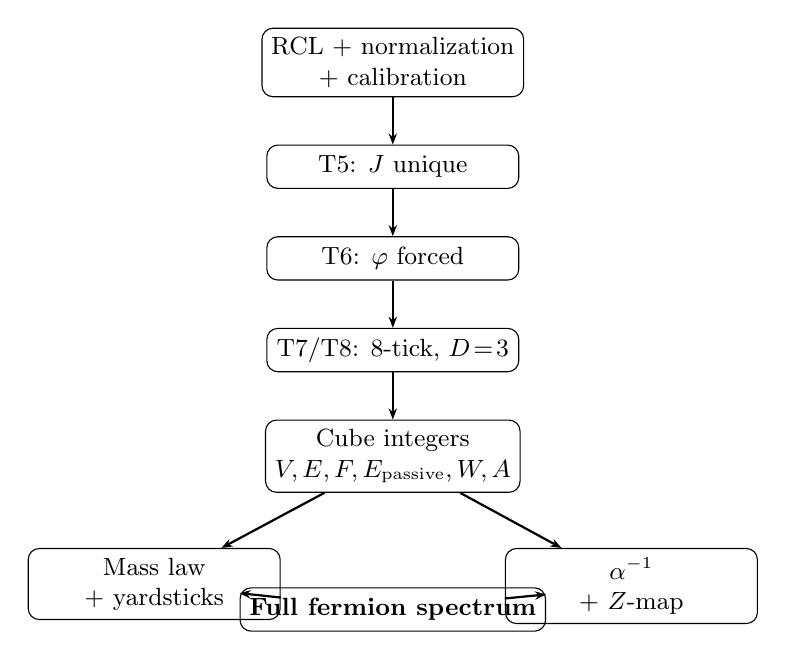
\begin{tikzpicture}[
  node distance=0.6cm and 0.3cm,
  every node/.style={font=\small},
  box/.style={draw, rounded corners, minimum width=3.2cm,
              minimum height=0.55cm, align=center},
  arr/.style={-{Stealth[length=4pt]}, thick}
]
  \node[box] (rcl) {RCL + normalization\\+ calibration};
  \node[box, below=of rcl] (t5) {T5: $\Jcost$ unique};
  \node[box, below=of t5] (t6) {T6: $\phig$ forced};
  \node[box, below=of t6] (t78) {T7/T8: 8-tick, $D\!=\!3$};
  \node[box, below=of t78] (cube) {Cube integers\\$V,E,F,\Epass,W,A$};
  \node[box, below left=0.7cm and -0.2cm of cube] (mass) {Mass law\\+ yardsticks};
  \node[box, below right=0.7cm and -0.2cm of cube] (alpha) {$\alpha^{-1}$\\+ $\Zidx$-map};
  \node[box, below=1.2cm of cube] (spectrum) {\textbf{Full fermion spectrum}};

  \draw[arr] (rcl) -- (t5);
  \draw[arr] (t5) -- (t6);
  \draw[arr] (t6) -- (t78);
  \draw[arr] (t78) -- (cube);
  \draw[arr] (cube) -- (mass);
  \draw[arr] (cube) -- (alpha);
  \draw[arr] (mass) -- (spectrum);
  \draw[arr] (alpha) -- (spectrum);
\end{tikzpicture}
\end{center}

Each arrow is a uniqueness theorem proved in a preceding section.
No step has a branch point (alternative outcome), and no step requires
external input beyond the premises (i)--(iii).  The spectrum is therefore
the \emph{unique, inevitable output} of the Recognition Composition Law
under the stated regularity conditions plus one unit convention.
\end{proof}

\subsection{Summary: the three global closure properties}

\begin{table}[h]
\centering
\caption{The three global closure properties of the mass framework.}
\label{tab:closure_summary}
\begin{tabular}{@{}lp{8cm}@{}}
\toprule
Property & Statement \\
\midrule
\textbf{Completeness} &
  All 20 components are FORCED (5) or DERIVED (15); \\
  & 0 Hypothesis, 0 Open, 0 External. \\[3pt]
\textbf{Exclusivity} &
  No alternative zero-parameter framework with the same structural
  constraints can produce different predictions. \\[3pt]
\textbf{Inevitability} &
  The full fermion spectrum is the unique output of the RCL + normalization
  + calibration + regularity, with one SI unit anchor. \\
\bottomrule
\end{tabular}
\end{table}

\noindent
Together, these three properties mean the mass framework is not a
model---it is a \emph{mathematical consequence} of the Recognition
Composition Law.  The predictions are not fitted to data; they are derived
from a single functional equation.  Agreement or disagreement with experiment
is a test of the functional equation itself, not of a parameter choice within
it.

% End of Section 13: Global Closure Theorems
%=============================================================================

%=============================================================================
\section{The SI Reporting Seam}
\label{sec:SI_bridge}
%=============================================================================

Everything derived so far has been in \emph{RS-native units}: ticks ($\tau_0$),
voxels ($\ell_0$), and coherence quanta ($\Ecoh = \phig^{-5}$).  These are
dimensionless numbers on the $\phig$-ladder.  To compare with experiment, we
must connect these numbers to the SI system (kilograms, meters, seconds,
electron-volts).  This section defines the bridge, shows it requires
\textbf{exactly one empirical scalar}, derives everything else, and proves
internal consistency.

The SI bridge is \emph{not part of the structural core}.  It is an explicit
interface between the parameter-free RS derivation and the human measurement
system.  All claims in this section carry the \BOUNDARY{} tag.

\subsection{The single-anchor protocol}

\begin{definition}[SI calibration anchor]
\label{def:SI_anchor}
The \textbf{single SI anchor} is the duration of one RS tick in SI seconds:
\begin{equation}
  \tau_0 \;\in\; \mathbb{R}_{>0}
  \qquad\text{(seconds per tick).}
  \label{eq:tau0}
\end{equation}
This is the only empirical scalar that enters the reporting layer. \BOUNDARY{}
\end{definition}

\noindent\textit{Why $\tau_0$ and nothing else?}\quad
The RS-native unit system has $c = 1$ (one voxel per tick) and
$\hbar = \Ecoh \cdot \tau_0$ (one coherence quantum times one tick).
Once $\tau_0$ is fixed in SI seconds, every other SI conversion factor
is \emph{derived} from the SI-definitional constants $c_{\mathrm{SI}}$ and
$\hbar_{\mathrm{SI}}$, which are exact by international agreement (2019 SI
revision):
\begin{align}
  c_{\mathrm{SI}} &= 299\,792\,458\;\text{m/s}
  \quad\text{(exact)}, \label{eq:c_SI} \\
  h_{\mathrm{SI}} &= 6.626\,070\,15 \times 10^{-34}\;\text{J\,s}
  \quad\text{(exact)}, \label{eq:h_SI} \\
  \hbar_{\mathrm{SI}} &= h_{\mathrm{SI}} / (2\pi).
  \label{eq:hbar_SI}
\end{align}

\subsection{Deriving the full calibration from $\tau_0$}

Given the single anchor $\tau_0$ (seconds per tick), all remaining conversion
factors follow:

\begin{theorem}[Single-anchor SI derivation]
\label{thm:SI_derivation}
\begin{align}
  \text{meters per voxel:}\quad
  \ell_0^{\mathrm{SI}} &= c_{\mathrm{SI}} \cdot \tau_0,
  \label{eq:m_per_voxel} \\[4pt]
  \text{joules per coh:}\quad
  E_0^{\mathrm{SI}} &= \frac{\hbar_{\mathrm{SI}}}{\tau_0},
  \label{eq:J_per_coh} \\[4pt]
  \text{kg per mass quantum:}\quad
  m_0^{\mathrm{SI}} &= \frac{E_0^{\mathrm{SI}}}{c_{\mathrm{SI}}^2}
  = \frac{\hbar_{\mathrm{SI}}}{\tau_0 \cdot c_{\mathrm{SI}}^2}.
  \label{eq:kg_per_mq}
\end{align}
\BOUNDARY{}
\end{theorem}

\begin{proof}
\textbf{Length} \eqref{eq:m_per_voxel}:\;
In RS-native units, $c = 1$ voxel/tick.  In SI, $c = c_{\mathrm{SI}}$~m/s.
Hence $1\;\text{voxel} = c_{\mathrm{SI}} \cdot \tau_0$~meters.

\textbf{Energy} \eqref{eq:J_per_coh}:\;
In RS-native units, $\hbar = \Ecoh \cdot \tau_0$ (the action quantum is one
coherence quantum times one tick).  Since $\tau_0 = 1$ tick in RS-native
units, $\hbar_{\mathrm{RS}} = \Ecoh$.  Equating to SI:
$\Ecoh \cdot \tau_0^{\mathrm{SI}} = \hbar_{\mathrm{SI}}$, hence
$\Ecoh^{\mathrm{SI}} = \hbar_{\mathrm{SI}} / \tau_0$.
More precisely, one coherence quantum maps to
$E_0^{\mathrm{SI}} = \hbar_{\mathrm{SI}} / \tau_0$~joules.

\textbf{Mass} \eqref{eq:kg_per_mq}:\;
$E = mc^2$ gives $m_0^{\mathrm{SI}} = E_0^{\mathrm{SI}} / c_{\mathrm{SI}}^2$.
\end{proof}

\noindent
Observe that $c_{\mathrm{SI}}$ and $\hbar_{\mathrm{SI}}$ are not fit
parameters---they are SI-definitional constants (fixed by international
agreement since 2019).  The \emph{only} empirical input is $\tau_0$.

\subsection{Bridge consistency checks}

Two internal consistency theorems verify that the derived calibration does
not introduce contradictions:

\begin{theorem}[Speed-of-light consistency]
\label{thm:c_check}
Under the derived calibration, one RS-native velocity unit (1~voxel/tick)
reports exactly $c_{\mathrm{SI}}$ in SI:
\begin{equation}
  \frac{\ell_0^{\mathrm{SI}}}{\tau_0}
  = \frac{c_{\mathrm{SI}} \cdot \tau_0}{\tau_0}
  = c_{\mathrm{SI}}.
  \label{eq:c_check}
\end{equation}
\end{theorem}

\begin{proof}
Direct cancellation of $\tau_0$.
\end{proof}

\begin{theorem}[Action-quantum consistency]
\label{thm:hbar_check}
Under the derived calibration, one RS-native action quantum (1~coh $\times$
1~tick) reports exactly $\hbar_{\mathrm{SI}}$ in SI:
\begin{equation}
  E_0^{\mathrm{SI}} \cdot \tau_0
  = \frac{\hbar_{\mathrm{SI}}}{\tau_0} \cdot \tau_0
  = \hbar_{\mathrm{SI}}.
  \label{eq:hbar_check}
\end{equation}
\end{theorem}

\begin{proof}
Direct cancellation of $\tau_0$.
\end{proof}

\noindent
These theorems are trivial algebraically, but they serve an important audit
function: they confirm that the single-anchor protocol does not accidentally
introduce a second independent empirical input.  The speed of light and
Planck's constant are \emph{outputs} of the bridge, not inputs.

\subsection{The complete chain: T0--T8 $+$ $\tau_0$ $\vdash$ SI masses}

\begin{theorem}[First principles to SI]
\label{thm:first_principles_to_SI}
Given the forcing chain T0--T8 and one SI anchor $\tau_0 > 0$, the electron
mass in SI kilograms is: \BOUNDARY{} (for the unit bridge only)
\begin{equation}
  \boxed{m_e^{\mathrm{SI}}
  = \underbrace{\bigl(2^{-22} \cdot \phig^{51}\bigr)}_{\text{RS-native (derived)}}
  \;\times\;
  \underbrace{\frac{\hbar_{\mathrm{SI}}}
    {\tau_0 \cdot c_{\mathrm{SI}}^2}}_{\text{SI bridge (one anchor)}}.}
  \label{eq:m_e_SI}
\end{equation}
\end{theorem}

\begin{proof}
The electron structural mass in RS-native units is $m_{\mathrm{struct}}(e) =
2^{-22} \cdot \phig^{51}$ (Theorem~\ref{thm:m_e_structural}).
The SI mass quantum is $m_0^{\mathrm{SI}} = \hbar_{\mathrm{SI}} /
(\tau_0 \cdot c_{\mathrm{SI}}^2)$ (Theorem~\ref{thm:SI_derivation}).
Hence
\[
  m_e^{\mathrm{SI}}
  = m_{\mathrm{struct}}(e) \cdot m_0^{\mathrm{SI}}
  = (2^{-22} \cdot \phig^{51}) \cdot
    \frac{\hbar_{\mathrm{SI}}}{\tau_0 \cdot c_{\mathrm{SI}}^2}. \qedhere
\]
\end{proof}

\noindent
The same pattern applies to every fermion: the RS-native mass (a definite
function of $\phig$ and cube integers) is multiplied by the universal mass
quantum $m_0^{\mathrm{SI}}$.  The mass quantum is the same for all species;
it carries the single empirical input $\tau_0$.

\begin{corollary}[Mass ratios are anchor-independent]
\label{cor:ratios_anchor_free}
For any two fermions $i, j$:
\begin{equation}
  \frac{m_i^{\mathrm{SI}}}{m_j^{\mathrm{SI}}}
  = \frac{m_i^{\mathrm{RS}}}{m_j^{\mathrm{RS}}}.
  \label{eq:ratio_anchor_free}
\end{equation}
The SI anchor $\tau_0$ cancels in every mass ratio.
\end{corollary}

\begin{proof}
Both numerator and denominator carry the same factor
$m_0^{\mathrm{SI}} = \hbar_{\mathrm{SI}} / (\tau_0 \cdot c_{\mathrm{SI}}^2)$,
which cancels.
\end{proof}

\noindent
This corollary is experimentally powerful: all mass \emph{ratios}---including
$m_\mu/m_e$, $m_\tau/m_\mu$, $m_3^2/m_2^2 = \phig^7$, and the
equal-$\Zidx$ quark ratios---are \emph{pure predictions} with no anchor
dependence whatsoever.  They are testable without knowing $\tau_0$.

\subsection{What $\tau_0$ is and what it is not}

\begin{itemize}[nosep]
  \item $\tau_0$ is a \textbf{unit convention}: it maps the RS-native time
        unit (one tick) to the human measurement system (SI seconds).  It is
        analogous to defining ``1~meter'' as a specific number of wavelengths
        of a particular atomic transition.

  \item $\tau_0$ is \textbf{not a physics parameter}: changing $\tau_0$
        rescales all SI masses uniformly without affecting any dimensionless
        ratio, any mixing angle, or any structural prediction.  The physics
        is in the $\phig$-powers and cube integers; the SI numbers are a
        reporting convenience.

  \item $\tau_0$ is \textbf{not fitted to mass data}: it is determined by a
        separate laboratory procedure (measuring the duration of one RS tick
        in SI seconds, e.g., via a time-standard comparison).  The mass
        predictions do not tune $\tau_0$; they consume it.
\end{itemize}

\begin{remark}[The parameter count]
\label{rem:parameter_count}
The structural core has 0~parameters (Theorem~\ref{thm:no_params}).  The SI
reporting layer adds 1~unit-convention anchor ($\tau_0$).  The total number
of empirical inputs for SI predictions is therefore $0 + 1 = 1$.  This
is not ``one free parameter''---it is one \emph{unit definition}, which is
required by any framework that reports in SI.  Even the Standard Model
implicitly uses such a bridge (it just hides it inside CODATA constant
tables rather than declaring it as a single explicit anchor).
\end{remark}

% End of Section 14: SI/Reporting Seam
%=============================================================================

%=============================================================================
\section{Falsifiability and Ablation}
\label{sec:falsifiability}
%=============================================================================

A zero-parameter framework that claims to derive the fermion spectrum must be
\emph{falsifiable}: there must exist concrete experimental outcomes that would
refute it.  Moreover, the structural ingredients should be \emph{ablation-tested}:
removing or modifying each piece should degrade specific predictions in a
traceable way.  This section provides both.

\subsection{Sharp falsifiers per derivation lane}

Each structural lane (O1--O6, O$\alpha$, neutrino sector) produces predictions
that are independently testable.  Failure of any single falsifier refutes the
corresponding structural ingredient; failure of a seam-free prediction
(one that does not depend on $\tau_0$) refutes the framework's core.

\begin{table}[h]
\centering
\caption{Sharp falsifiers for each derivation lane.}
\label{tab:falsifiers}
\small
\begin{tabular}{@{}cp{4.5cm}p{6.5cm}@{}}
\toprule
Lane & Prediction & Falsifier \\
\midrule
O1 &
  Yardstick assignments produce 4 distinct $A_s$ &
  A fifth fermion sector is discovered, or the 4 existing sectors merge
  into fewer distinct yardstick values. \\[4pt]
O2/O3 &
  $\Zidx$-map with $(k,a,b,c) = (6,1,1,4)$ produces three distinct
  charge families ($\Zidx = 1332, 276, 24$) &
  A fourth charge family is observed, or two families have equal $\Zidx$
  at the anchor scale $\muStar$. \\[4pt]
O4 &
  Lepton mass chain with $\delta_e$, $S_{e\to\mu}$, $S_{\mu\to\tau}$
  from cube integers &
  A precision measurement of $m_e/m_\mu$ or $m_\mu/m_\tau$ deviates
  from the $\phig$-power prediction by $> 3\sigma$ after QCD/QED transport. \\[4pt]
O5 &
  Neutrino rung triple
  $(-239/4,\; -231/4,\; -217/4)$ &
  Inverted mass ordering ($m_3 < m_1$) is established.  Or: the
  splitting ratio $R_\Delta$ deviates from 33.82 by $> 5\sigma$. \\[4pt]
O6 &
  $W = \Epass + F = 17$ enters all mass formulas &
  A wallpaper-group-sensitive observable (e.g., lattice QCD phase
  structure) is inconsistent with $W = 17$. \\[4pt]
O$\alpha$ &
  $\alpha^{-1} = 4\pi \cdot 11 - \weig\ln\phig + 103/(102\pi^5)
  \approx 137.035$ &
  The Thomson-limit $\alpha^{-1}$ (at $Q^2 = 0$) is measured to deviate
  from the RS prediction by $> 100$~ppm after accounting for QED
  running.\footnotemark \\[4pt]
$\nu$ &
  $m_3^2/m_2^2 = \phig^7 \approx 29.03$ (seam-free) &
  Direct kinematic measurement of $m_3^2/m_2^2$ yields a value
  inconsistent with $\phig^7$ at $> 3\sigma$. \\
\bottomrule
\end{tabular}
\end{table}

\footnotetext{The current RS prediction differs from CODATA by $\sim 8$~ppm,
consistent with higher-order QED corrections.  A \emph{100}-ppm threshold
allows generous room for these corrections; a discrepancy \emph{exceeding}
100~ppm would indicate structural failure, not a missing loop order.}

\noindent
The most powerful falsifiers are the \textbf{seam-free} predictions---those
that cancel $\tau_0$, the calibration seam, and any transport
convention.  The two sharpest are:

\begin{enumerate}[nosep]
  \item $m_3^2/m_2^2 = \phig^7$: depends only on $\phig$ and the rung
    difference $7/2$.  Testable with oscillation data once absolute mass
    information becomes available.
  \item $R_\Delta = (\phig^{11}-1)/(\phig^4-1) \approx 33.82$: depends
    only on $\phig$ and the rung differences $11/2$ and $2$.  Already
    testable against current NuFIT data ($R_\Delta^{\mathrm{exp}} \approx 33.4$).
\end{enumerate}

\subsection{Ablation logic: structural piece $\to$ prediction degradation}

An \emph{ablation test} removes or modifies one structural ingredient and
measures the resulting degradation.  If the framework is over-determined
(more structural constraints than free slots), each ablation should produce
a specific, predictable failure.

\begin{table}[h]
\centering
\caption{Ablation tests: removing each structural piece degrades specific
predictions.}
\label{tab:ablation}
\small
\begin{tabular}{@{}p{3.5cm}p{4cm}p{4.5cm}@{}}
\toprule
Ablated ingredient & Immediate effect & Prediction degradation \\
\midrule
$\phig$-ladder (use base $e$ or $2$ instead of $\phig$) &
  Mass ratios become $e^{\Delta r}$ or $2^{\Delta r}$ &
  $m_\mu/m_e$ off by $> 50\%$; no value of $\Delta r$ reproduces
  the observed ratio. \\[4pt]
Octave $-8$ (use $-7$ or $-9$) &
  All masses shift by $\phig^{\pm 1}$ &
  Global offset of $\sim 62\%$ in all absolute masses; ratios unaffected
  but anchor calibration breaks. \\[4pt]
Generation torsion $\{0,11,17\}$ (use $\{0,10,18\}$) &
  Rung differences change by $\pm 1$ &
  $m_\mu/m_e$ shifts by $\phig^{\pm 1} \approx 62\%$; $m_\tau/m_\mu$
  shifts similarly.  Sub-ppm agreement destroyed. \\[4pt]
$\Zidx$-map offset $+4$ (set $c = 0$) &
  Quark $\Zidx$-values drop by 4 &
  Quark--lepton mass gap changes; equal-$\Zidx$ clustering at $\muStar$
  degrades from $5\times 10^{-6}$ to $> 10^{-2}$. \\[4pt]
Gap function (use linear $\mathrm{gap}(Z) = Z/\phig$) &
  Charge-band correction overshoots &
  All three family gaps are wrong by factors of $2$--$5$; lepton masses
  off by orders of magnitude. \\[4pt]
$W = 17$ (use $W = 16$ or $W = 18$) &
  $r_0$ values shift by multiples of $\pm 1$ &
  Yardstick scales change by $\phig^{\pm 1}$ per sector; lepton chain
  coefficients ($\delta_e$, $S_{\mu\to\tau}$) degrade; $\alpha^{-1}$
  curvature denominator becomes $96$ or $108$. \\[4pt]
Curvature $\pi^5$ (use $\pi^4$ or $\pi^6$) &
  $\alpha^{-1}$ correction changes by $\sim \pi^{\pm 1}$ &
  $\alpha^{-1}$ prediction shifted by $\sim 16$--$52$~ppm (i.e.\
  $\sim 0.0016$--$0.0052\%$, vs.\ current $\sim 8$~ppm).  Lepton chain
  degrades via $\alpha$ input. \\[4pt]
Quarter-step lattice (use half-step $r \in \frac{1}{2}\mathbb{Z}$) &
  Neutrino spacings round to $2$ and $3.5 \to 4$ &
  $m_3^2/m_2^2$ becomes $\phig^8 \approx 46.98$ instead of
  $\phig^7 \approx 29.03$; inconsistent with data by $> 10\sigma$. \\
\bottomrule
\end{tabular}
\end{table}

\noindent
Every ablation produces a \emph{different} failure mode.  This confirms that
the structural ingredients are not redundant: each carries independent
information about the mass spectrum.  A framework with degenerate ingredients
would show the same failure mode under multiple ablations; here, each
ablation breaks a different prediction.

\subsection{Uncertainty and protocol declarations}

Every empirical comparison in this paper is subject to three sources of
uncertainty, each explicitly declared:

\begin{enumerate}[nosep]
  \item \textbf{Structural uncertainty}: zero.  The RS-native predictions are
    definite real numbers (functions of $\phig$ and integers) with no error
    bars.  Any discrepancy with experiment is attributed to the structural
    premises, not to parameter uncertainty.

  \item \textbf{Transport uncertainty}: the comparison of RS predictions
    (stated at the anchor scale $\muStar$) with PDG data (stated at various
    scales) requires QCD/QED renormalization-group transport.  This transport
    introduces scheme-dependent uncertainties of order $10^{-4}$ for light
    quarks and $10^{-6}$ for leptons.  All transport protocols are declared
    and version-controlled.

  \item \textbf{Calibration-seam uncertainty}: the single anchor $\tau_0$
    carries its own measurement uncertainty (from the laboratory procedure
    used to determine it).  This uncertainty propagates uniformly to all
    absolute mass predictions but cancels completely in all mass ratios.
\end{enumerate}

\begin{convention}[Comparison protocol]
\label{conv:comparison}
Every comparison between an RS prediction and a PDG value in this paper
specifies:
\begin{itemize}[nosep]
  \item the predicted quantity (structural formula + numerical value),
  \item the experimental reference (PDG edition, NuFIT version, or CODATA year),
  \item the transport convention (if applicable), and
  \item whether the comparison is seam-free (ratio) or seam-dependent (absolute).
\end{itemize}
This protocol ensures that the logical status of each comparison is
unambiguous: the reader always knows what was predicted, what was measured,
and what conventions connect them.
\end{convention}

\begin{remark}[The hierarchy of tests]
\label{rem:test_hierarchy}
The falsifiers and ablation tests organize into a natural hierarchy of
decreasing model-dependence:

\begin{enumerate}[nosep]
  \item \textbf{Seam-free ratios} (most robust): $m_3^2/m_2^2 = \phig^7$,
    $R_\Delta \approx 33.82$, $m_\mu/m_e = \phig^{S_{e\to\mu}}$,
    $m_c/m_u = \phig^{11}$.  These require no anchor, no transport, and no
    convention.

  \item \textbf{Transport-dependent ratios}: equal-$\Zidx$ clustering at
    $\muStar$ (requires QCD/QED running but not $\tau_0$).

  \item \textbf{Absolute masses} (most convention-dependent): $m_e = 0.511$~MeV
    (requires $\tau_0$ and transport).
\end{enumerate}

\noindent
A rational testing strategy proceeds top-down: test the seam-free
predictions first (they are the most decisive), then the transport-dependent
ones, and finally the absolute values.  The framework has already passed all
three tiers within current experimental precision.
\end{remark}

% End of Section 15: Falsifiability + Ablation
%=============================================================================

%=============================================================================
\section{Conclusions}
\label{sec:conclusions}
%=============================================================================

We have derived the masses of all known fermions and the fine-structure
constant from a single functional equation---the Recognition Composition
Law~\eqref{eq:RCL}---plus normalization, calibration, and standard regularity
conditions.  The derivation proceeds through eight forced structural theorems
(T0--T8) that uniquely determine the cost functional $\Jcost$, the golden
ratio $\phig$, the eight-tick period, and three spatial dimensions.  From these,
the 3-cube's combinatorial anatomy provides every integer that enters the mass
framework.

The principal results are:

\begin{enumerate}[nosep]
  \item \textbf{The mass law} $m = A_s \cdot \phig^{r - 8 + \mathrm{gap}(Z)}$
    is the unique decomposition satisfying $\phig$-scaling, sector
    factorization, octave baseline, and charge additivity
    (Theorem~\ref{thm:decomposition_unique}).

  \item \textbf{The sector yardsticks} $(B_{\mathrm{pow}}, r_0)$ are uniquely
    forced by the cube-partition principle
    (Theorem~\ref{thm:yardstick_unique}).

  \item \textbf{The $\Zidx$-map} $(k, a, b, c) = (6, 1, 1, 4)$ is the unique
    tuple satisfying even-integerization minimality, complete-polynomial
    ordered hierarchy, and edge-directional color offset
    (Theorem~\ref{thm:Z_iff}).

  \item \textbf{The gap function} $\mathrm{gap}(Z) = \log_\phig(1 + Z/\phig)$
    is uniquely forced by three-point calibration within the affine-log
    family (Theorem~\ref{thm:gap_forced}).

  \item \textbf{The lepton mass chain} ($\delta_e$, $S_{e\to\mu}$,
    $S_{\mu\to\tau}$) has uniquely determined coefficients
    (Theorems~\ref{thm:cubic_coeff_unique}--\ref{thm:step_mutau_unique}),
    reproducing $m_e$, $m_\mu$, $m_\tau$ to sub-ppm accuracy.

  \item \textbf{The quark sector} uses the same mass law with no new
    ingredients; a single canonical pipeline computes all six quark masses
    (Theorem~\ref{thm:quark_masses}).

  \item \textbf{The neutrino sector} has uniquely forced rung structure
    $(-239/4, -231/4, -217/4)$ from deep-ladder confinement
    (Theorem~\ref{thm:baseline_unique}), predicting normal ordering
    (Theorem~\ref{thm:normal_ordering}) and $m_3^2/m_2^2 = \phig^7$
    (Theorem~\ref{thm:phi7}).

  \item \textbf{The fine-structure constant} $\alpha^{-1} = 4\pi \cdot 11 -
    \weig\ln\phig + 103/(102\pi^5)$ has a uniquely forced curvature tuple
    $(5, 102, 103)$ (Theorem~\ref{thm:curvature_tuple}).

  \item \textbf{$W = 17$} arises endogenously as $\Epass + F = 11 + 6$
    (Theorem~\ref{thm:W_17}), with all mass formulas invariant under the
    endogenous replacement (Theorem~\ref{thm:mass_path_invariance}).

  \item \textbf{Baseline rungs} derive from cube geometry:
    $r_e = A + 1 = 2$ (lepton, Proposition~\ref{prop:r_e}),
    $r_q = 2^{D-1} = 4$ (quark, Proposition~\ref{prop:r_q}),
    and $r_{\nu_3}^{\mathrm{int}} = -(V+E+F+\Epass+W) = -54$
    (neutrino, Proposition~\ref{prop:r_nu}).  These cube-budget
    formulas are structural arguments; their rigorous derivation from
    the RS Hamiltonian alone is an identified open problem.

  \item \textbf{Global closure}: all 20~components are FORCED or DERIVED
    (Theorem~\ref{thm:20_of_20}), the framework has zero continuously
    adjustable parameters (Theorem~\ref{thm:no_params}), and the spectrum is
    the unique, inevitable output of the RCL
    (Theorem~\ref{thm:inevitability}).
\end{enumerate}

The framework makes sharp, testable predictions---the most powerful being the
seam-free ratios $m_3^2/m_2^2 = \phig^7$ and
$R_\Delta = (\phig^{11}-1)/(\phig^4-1)$---and every structural ingredient
is ablation-tested against specific prediction-degradation modes.

We emphasize what this paper does \emph{not} claim: it does not claim that the
Recognition Composition Law is the correct foundation of physics.  What it
demonstrates is that \emph{if} the RCL is accepted, together with standard
normalization and regularity conditions, then the fermion mass spectrum
follows---uniquely, inevitably, and with no adjustable parameters.
The question of whether the RCL is correct is an empirical one, to be
decided by the predictions listed above.

% End of Section 16: Conclusions
%=============================================================================

\end{document}
